\documentclass[british]{ntnuthesis}

\title{Parallel Processing and Anomaly Detection of DAS Data using Autoencoders: Enhancing Efficiency in Large-Scale Sensor Data Analysis}
\shorttitle{Parallel Processing and Anomaly Detection on DAS data}
\author{Jørgen Aleksander Fagervik \\
        Supervisor: Ole Jakob Mengshoel \\
        Co-supervisor: Anne Cathrine Elster}
\shortauthor{J. A. Fagervik}
\date{CC-BY \ntnuthesisdate}

\addbibresource{thesis.bib}


% From https://www.overleaf.com/learn/latex/Glossaries

\makeglossaries % Prepare for adding glossary entries

\newglossaryentry{julia}
{
        name=Julia,
        description={Is an all-purpose programming language specially suited for
scientific computing}
}

\newglossaryentry{python}
{
        name=Python,
        description={Is an all-purpose general programming language suited for scripting, data-science and web applications}
}

\newglossaryentry{llvm}
{
        name=LLVM,
        description={Low Level Virtual Machine, better known as LLVM, is a project trying to provide a modern, SSA-based compilation strategy capable of supporting both static and dynamic compilation of arbitrary programming languages \cite{llvm}}
}

\newglossaryentry{fftw}
{
        name=FFTW,
        description={Fastest Fourier Transform in the West is one of the most famous implementations of the \acrshort{dft} algorithm. It is specialized for running on \acrlong{cpu}s}
}

\newglossaryentry{relu}
{
    name=ReLU,
    description={Rectified Linear Unit is one of the most commonly used activation functions within \acrshort{dnn}s}
}

\newglossaryentry{bibliography}
{
        name=bibliography,
        plural=bibliographies,
        description={A list of the books referred to in a scholarly work,
typically printed as an appendix}
}

\newglossaryentry{maths}
{
    name=mathematics,
    description={Mathematics is what mathematicians do}
}
\newglossaryentry{pubdas}
{
    name=PubDAS,
    description={A PUBlic Distributed Acoustic Sensing Datasets Repository for Geosciences}
}

\newglossaryentry{idun}{
    name=IDUN,
    description={The Idun cluster is a project between NTNU's faculties and the IT division that aims at providing a high-availability and professionally administrated compute platform for NTNU}
}

\newglossaryentry{svm}
{
    name=Support Vector Machine,
    description={Common machine learning technique}
}




% --------------------
% ----- Acronyms -----
% --------------------

\newacronym{ntnu}{NTNU}{Norwegian University of Science and Technology}
\newacronym{ai}{AI}{Artificial Intelligence}
\newacronym{ast}{AST}{Abstract Syntax Tree}
\newacronym{mb}{MB}{Megabyte}
\newacronym{gb}{GB}{Gigabyte}
\newacronym{tb}{TB}{Terrabyte}
\newacronym{ml}{ML}{Machine Learning}
\newacronym{fft}{FFT}{Fast Fourier Transform}
\newacronym{rfft}{RFFT}{Fast Fourier Transform for Real Numbers}
\newacronym{dft}{DFT}{Discrete Fourier Transform}
\newacronym{mpi}{MPI}{Message-passing interface}
\newacronym{ram}{RAM}{Random-access memory}
\newacronym{gcd}{GCD}{Greatest Common Divisor}
\newacronym{hpc}{HPC}{High Performance Computing}
\newacronym{api}{API}{Application programm interface}
\newacronym{gpu}{GPU}{Graphics processing unit}
\newacronym{tpu}{TPU}{Tensor processing unit}
\newacronym{cpu}{CPU}{Central processing unit}
\newacronym{das}{DAS}{Distributed accoustic sensoring}
\newacronym{ann}{ANN}{Artificial neural network}
\newacronym{cnn}{CNN}{Convolutional neural network}
\newacronym{rnn}{RNN}{Recurrent Neural Network}
\newacronym{dnn}{DNN}{Deep Neural Network}
\newacronym{repl}{REPL}{Read-eval-print loop}
\newacronym{lstm}{LSTM}{Long short-term memory}
\newacronym{jit}{JIT}{Just-in-time}
\newacronym{hdf}{HDF}{Hierarchical Data Format}
\newacronym{hdf5}{HDF5}{Hierarchical Data Format version 5}
\newacronym{sisd}{SISD}{Hierarchical Data Format version 5}
\newacronym{simd}{SIMD}{Single instruction, multiple device}
\newacronym{misd}{MISD}{Multiple instructions, single device}
\newacronym{mimd}{MIMD}{Multiple intstructions, multiple device}
\newacronym{spmd}{SPMD}{Single program, multiple device}
\newacronym{cgf}{NTNU CGF}{NTNU Centre for Geophysical Forecasting}
\newacronym{posix}{POSIX}{Portable Operating System Interface}
\newacronym{asn}{ASN}{ALCATEL SUBMARINE NETWORKS}
\newacronym{dsp}{DSP}{Digital Signal Processing}
\newacronym{adam}{ADAM}{Adaptive Moment estimation}
\newacronym{sgd}{SGD}{Stochastic Gradient Descent}
\newacronym{gru}{GRU}{Gated Recurrent Unit}
\newacronym{llm}{LLM}{Large Language Model}
\newacronym{sota}{SOTA}{State of the Art}
\newacronym{dl}{DL}{Deep Learning}
\newacronym{vae}{VAE}{Variational Auto Encoder}
\newacronym{mae}{MAE}{Mean Absolute Error}
\newacronym{mse}{MSE}{Mean Squared Error}
\newacronym{gan}{GAN}{Mean Squared Error}
\newacronym{dbscan}{DBSCAN}{Density-Based Spatial Clustering of Applications with Noise}
\newacronym{adagrad}{AdaGrad}{Adaptive Gradient Algorithm}
\newacronym{fir}{FIR}{Finite Impulse Response}
\newacronym{roi}{ROI}{Range of Interest} % add glossary and acronym lists before document
\usepackage{listings}
\usepackage[table,xcdraw]{xcolor}
\usepackage{siunitx}
\usepackage{multirow}
\usepackage{pgfplots}
\usepackage{algorithm}
\usepackage{algpseudocode}
\usepackage{textcomp}
\usepackage{tikz}
\usepgfplotslibrary{groupplots}
\usepackage{booktabs}
\usepackage{colortbl}
\usepackage{array}
\usepackage{makecell}
\usepackage{xcolor}
\usepackage{caption}

% Define a custom color for the caption background
\definecolor{captionbg}{RGB}{240,240,240}
\definecolor{captiontext}{RGB}{0,0,0}
\definecolor{captionframe}{RGB}{100,100,100}

\newcommand{\mycomment}[1]{}
% Define a custom caption style
\DeclareCaptionFormat{thesiscaption}{%
    \begin{tikzpicture}
    \node[inner sep=10pt, fill=captionbg, draw=captionframe, line width=0.5pt, rounded corners] {%
        \parbox{\dimexpr\textwidth-20pt\relax}{%
            \textbf{\color{captiontext}#1#2}%
            \par\vskip2pt%
            \color{captiontext}#3%
        }%
    };
    \end{tikzpicture}%
}

% Apply the custom style to listings and figures
\captionsetup[lstlisting]{format=thesiscaption, labelfont={bf}, textfont={}, justification=justified, singlelinecheck=false}

% Define Julia style
\lstdefinelanguage{Julia}{
  keywords={abstract, break, case, catch, const, continue, do, else, elseif, end, export, false, for, function, global, if, import, in, macro, module, otherwise, quote, return, true, try, using, while, type, mutable, struct, @inline, @simd, @time, @btime, @layer, @functor, @error, @warn, @show, @inbounds, @kwdef, @view, @layout, @gif,
  Real, Integer, Int, Int8, Int16, Int32, Int64,
  String, AbstractString,
  DateTime, Second, Minute, Hour, Date,
  Bool, Tuple, Matrix, Dict, Set, Vector, AbstractArray, AbstractVector, AbstractMatrix,
  AbstractFloat, Float, Float8, Float16, Float32, Int64,
  },
  sensitive=true,
  comment=[l]\#,
  morecomment=[s]{\#=}{=\#},
  morestring=[b]",
}

\definecolor{backcolour}{rgb}{0.99,0.99,0.99}
\definecolor{codegreen}{rgb}{0,0.6,0}

% Define a custom style
\lstdefinestyle{dasstyle}{
    backgroundcolor=\color{backcolour},   
    commentstyle=\color{codegreen},
    basicstyle=\ttfamily\footnotesize,
    breakatwhitespace=false,         
    breaklines=true,                 
    keepspaces=true,                 
    numbers=left,
    frame=single,
    numbersep=5pt,                  
    showspaces=false,                
    showstringspaces=false,
    showtabs=false,                  
    tabsize=2,
}

% Define colors for the command prompt
\definecolor{promptcolor}{rgb}{0.5,0,0}
\definecolor{commandcolor}{rgb}{0,0,0.5}

% Configure the listing style for shell commands
\lstdefinestyle{shellcommand}{
  basicstyle=\ttfamily\small,
  breaklines=true,
  captionpos=t,
  commentstyle=\color{promptcolor},
  keywordstyle=\color{commandcolor},
  stringstyle=\color{commandcolor},
  numbers=none,
  numbersep=5pt,
  numberstyle=\tiny\color{black},
  frame=single,
  framesep=5pt,
  xleftmargin=15pt,
  framexleftmargin=15pt,
  backgroundcolor=\color{gray!10},
  showspaces=false,
  showstringspaces=false,
  showtabs=false,
  tabsize=2,
  breakatwhitespace=false,
  escapeinside={(*@}{@*)},
}

% Use \lstset to make myStyle the global default
\lstset{style=dasstyle}

\begin{document}


\begin{titlepage}
\newgeometry{left=1.6in, right=2in}
\vspace*{1.5cm}

\noindent  \textcolor{gray}{\large Jørgen Aleksander Fagervik} \\
\vspace{1cm}

\noindent \textbf{\Large Parallel Processing and Autoencoder based Anomaly Detection of Distributed Acoustic Sensing Data} \\
\vspace{0.5cm}

\noindent {Designing Scalable Programs for Enhanced Efficiency in Large-Scale \acrshort{das} Data Processing and  Analysis} \\



\vspace{7cm}
\noindent Master's thesis in Computer Science \\
Supervisor: Ole Jakob Mengshoel \\
Co-supervisor: Anne Cathrine Elster \\
September 2024 \\

\vspace{0.2cm}
\noindent Norwegian University of Science and Technology \\
Faculty of Information techonolgy and electrical engineering \\
Department of Computer Science (IDI) \\

\begin{figure}[h]

\includegraphics[scale=0.5]{figures/ntnu.png}
\end{figure}
\end{titlepage}
\restoregeometry
\myemptypage 

\chapter*{Preface}

The beginning of the end. Six years have gone since I started university to pursue my passion. Little did I know what this years would hold, all the friends and people I'd meet, and all the new information I'd learn. I want to reminisce a bit about my journey towards where I am today. \\

I'd like to start off by saying that these years has had me feeling all kinds of emotion. From the happiest moments to the darkest of days. In the end I'm finishing my degree not only as a more proficient engineer, researcher and developer, but also as a more informed and well of human being. \\

I decided ot study computer science at the age of 12. I started of with simple webdesign and Python development, but also dabbled in game programming with the Unity engine. I became a part of Revolve NTNU during my first year, where I learnt a lot, not only about software tools like Git, JIRA and Confluence for documentation, but also software development as a whole. \\

I didn't exactly know what aspect of computer science I wanted to study, so in the en I forged my own path, trying to bridge the gap between HPC and AI. \\

I decided to 

I want to give a huge

\chapter*{Abstract}

Signal processing and \acrfull{ai} has become .

Parts of this thesis are taken from or based on my submitted project assignment in the subject TDT4501 with the title "Parallel DAS Processing: Julia is all you need".
\chapter*{Sammendrag}

Distribuert akustisk sensing (DAS) har blitt en utbredt teknologi det siste tiåret, men de nåværende metodene for prosessering og anomalideteksjon prioriterer ofte nøyaktighet fremfor effektivitet. Denne oppgaven tar for seg utfordringen med å effektivt prosessere DAS-data samtidig som man opprettholder effektive evner for anomalideteksjon. Vi undersøker parallellprosesseringsmetoder for storskala, tettprøvet DAS-data og utforsker anvendelsen av kompakte autoenkodere for rask anomalideteksjon.

Vi presenterer to verktøy: Judas, en pakke for effektiv innlasting og prosessering av DAS-data, og TinyDAS, et skalerbart rammeverk for opplæring av autoenkodere og utføring av anomalideteksjon. Disse verktøyene har som mål å redusere databehandlingsressurser og prosesseringstid betydelig for håndtering av DAS-data. Vi validerer disse programmene ved å bruke både proprietære og åpne DAS-datasett, med fokus på overvåking av jernbane og jordskjelvdeteksjon.

Vår forskning viser at minnekartlegging kan redusere minnekravene for DAS-databehandling betraktelig. I motsetning til eksisterende metoder som laster hele datasett inn i minnet, benytter vår teknikk distribuert binær filsplitting og behovsstyrt innlasting, noe som muliggjør effektiv håndtering av storskala DAS-data med minimal minnebruk. Videre viser vi at inferens i halv presisjon på en kompakt konvolusjonsbasert autoenkoder med bare 46k parametere kan oppdage anomalier i store matriser med 86\% nøyaktighet på bare 5,5 ms.

Dette arbeidet fremmer mer effektive teknikker for behandling av DAS-data, noe som kan være til nytte for ulike bransjer som benytter DAS-teknologi, inkludert infrastrukturovervåking og geofysisk prognosering. Ved å forbedre databehandlingsmetoder og fremme effektivt design av autoenkodere, baner vårt arbeid ved NTNU Senter for Geofysisk Prognosering vei for mer utbredte og ressursvennlige anvendelser av DAS-teknologi i sanntidsscenarioer.



\tableofcontents
\listoffigures
\listoftables
\lstlistoflistings

\printglossary[type=\acronymtype] % Print acronyms
\printglossary                    % Print glossary

\chapter{Introduction}
\label{chap:introduction}

This opening chapter presents the background and our motivation for this project, discusses current challenges, highlights this thesis's goals and contributions, and provides a chapter overview.

\section{Motivation}

Digital signal processing has over the last 100 years gone from almost non-existent to utmost critical importance. By processing signal data, one can get access to all kinds of information, music, movement and locations. There are tons of different devices for recording signals from the environments. From more well known ones such as microphones and sensors, to less commercial technologies.

The world of digital signal processing is nothing new to academia, and computer science in general. Some of the most magnificent and trailblazing algorithms, like the \acrfull{dft} algorithm revolve around solving problems revolving around these data. With more and more sensors being used around us, as well as the increasing amount of data stored, the larger the need for processing and interpreting this data has become. 
\acrfull{das} is a rather new technology that allows for real-time analysis over fiber-optical cables, and gives us highly sensitive senor data to work with. \acrshort{das} has gained more recognition. \\

It is hard to underestimate the impact \acrshort{ai} has had upon the general population this last couple of years. Ever since OpenAI released ChatGPT the 30th of november 2022 \cite{chatgpt} the amount of \acrshort{ai} technology and applications has exploded, not only large language models (\acrshort{llm}), but other domains have garnered attention as well. \acrshort{llm}s made \acrfull{rnn} more popular than they had been for a while. These models are good at remembering information, making current desicions based on previous ones. \\ 

\acrshort{das} technology in itself has now started garnering attention for research, and several papers have previously studied  how one can process this data. \acrshort{ai} and \acrshort{ml} models have been constructed for looking at time series data, and analyzing sensor data, although several of theses have studied .  Only recently has \acrshort{ai}

Anomaly detection on \acrshort{das} data 

Unsupervised learning has in later years returned after the explosion of generatiive models. They are well suited for detecting novel anomalies \cite{wei2022lstmautoencoder} \cite{srivastava2016unsupervised} and do not require labeling of data, something that can rather dificult on DAS data. Both GANs, AE, and LSTM VAE have been proven to have good metrics for determining anomalies. 


Python has for a long been the \textit{de-facto standard} language both for \acrshort{ai}, \acrshort{ml} and data analysis. All kinds of heavy pre-processing of data before training the data is being written in C or C++ or other more performant languages.    




Previous work on this data (see \cite{projthesis}) revolved around processing \acrshort{hdf5} files as fast and efficient as possible, trying to parallellize already existent code, and take advantage of newer technologies, such as Julia.

\subsection{NTNU SFI Center for Geophysical Forecasting}



We hereby present \texttt{JudasNET}, a LSTM VAE network written in Julia for anomaly detection on \acrshort{das} data. Additionally, we present \texttt{Judas - (Julia \& DAS)}, a Julia package containing functions for parsing HDF5 files, signal processing methods specifically for DAS sensor data, as well as functions for training, inference and utilities for AI models related to DAS data. As a sideeffect, we also show how Julia can be used effectively within multiple different fields to enable , and be easily tuned to their needs,
%\section{Goals}

Given the vast scope and multiple facets of our project, it is important to clarify the specific objectives we aim to achieve with this thesis. Our goals are as follows:

\begin{enumerate}
    \item \textbf{Evaluating Julia for Big Data Science Applications}: Determine whether Julia is a suitable programming language for big data, data science and \acrshort{ai} applications
    \item \textbf{Assessing Autoencoders for Anomaly Detection in \acrshort{das} Data}: Evaluate the effectiveness of autoencoders in detecting anomalies within \acrshort{das} data, both in online and offline data.
    \item \textbf{Open Source Contributions for \acrshort{das}}: Contribute to the open-source community, particularly with tools and resources that are beneficial to members of \acrshort{cgf}.
\end{enumerate}


\subsection{Research Questions}

In addition to our goals, the following are a set of research questions we want answers to by the end of the thesis:

\begin{enumerate}
    \item \textbf{Scalability and Parallelization in \acrshort{das} Data Processing}: Can we develop a program that is both scalable and parallelizable for processing and training large \acrshort{hdf5} files?
    \item \textbf{Float16 Processing on \acrshort{das} data}: Can we reduce the precision of \acrshort{das} data to enable faster model training and inference without sacrificing performance?
\end{enumerate}

\section{Research Questions and Contributions}
\label{intro:contribs}

The following list provides the research questions of this thesis: 

\begin{enumerate}
    \item How do the spatial characteristics of \acrshort{das} data impact the performance of autoencoders for anomaly detection?
    \item What autoencoder architectures are most effective for anomaly detection in \acrshort{das} data when computational resources can be limited?
    \item What preprocessing techniques can optimize the efficiency-accuracy trade-off in anomaly detection of \acrshort{das} data?
\end{enumerate}

In this thesis, we study processing and autoencoder-based anomaly detection using \acrshort{das} data. Our work has led to several contributions, including:

\begin{itemize}
    \item \textbf{Autoencoder based anomaly detection}: We compare the effectiveness of different autoencoders for anomaly detection on dense \acrshort{das} data. In particular, we explore the spatial characteristics of in \acrshort{das} data.
    \item \textbf{Julia for data science and \acrshort{ai}}: We evaluate Julia as a programming language for developing high-performance applications and \acrshort{ai} programming.
    \item \textbf{Software}: The following software has been produced as a part of this thesis:
    \begin{itemize}
        \item \textbf{Judas}: A software package developed in Julia for processing \acrshort{das} data. Initially introduced in our project thesis \cite{projthesis}, Judas is now fully operational but only available for members of \acrshort{cgf}. 
        \item \textbf{TinyDAS}: An open-source program written in Python, specifically designed for training and evaluation of autoencoder models, as well as performing anomaly detection on \acrshort{das} data \footnote{\url{github.com/Jafagervik/TinyDAS}}. This program contains code and hyperparameters for 4 different autoencoders.  We establish how Tinygrad \cite{tinygrad} as a software package can be used to create hardware agnostic \acrshort{ai} programs that are scalable across multiple accelerators without changing source code. 
        \item \textbf{JudasNET}: An open-source repository with examples of autoencoders written in Julia \footnote{\url{github.com/Jafagervik/JudasNET}}.
    \end{itemize}
\end{itemize}

Overall, we seek to improve \acrshort{das} data processing and compare the effectiveness of smaller autoencoder models for anomaly detection on this data. In particular, we hope that members of \acrshort{cgf} can use and improve these tools to further \acrshort{das} research.
\section{Thesis outline}

The following list is an outline over the rest of the thesis, and what will be presented for each chapter. \\

%\textbf{Chapter 1: Introduction} - We present the problems, what we want to find out and our motivation for this project. \\

\textbf{Chapter 2: Background and Related Work} - We cover theory regarding \acrshort{das} processing techniques, both relevant \acrshort{dl} architectures and their applications to our problems, as well as some introduction to applicable signal processing techniques. Finally, we discuss relevant literature and work.  \\

\textbf{Chapter 3: Method} - We cover all our practical work and implementation decisions of both programs, including program design, data processing methods, and network architectures. \\

\textbf{Chapter 4: Experiments} - We present our experiments, covering datasets, the experiments scopes, as well as evaluation metrics and experiment setup. \\

\textbf{Chapter 5: Experimental Results} - We present our results from the experiments conducted in the Chapter 4. \\

\textbf{Chapter 6: Discussion} - We discuss the overall findings and results of our experiments. Furthermore, we discuss the current capabilities of our programs, including limitations, and answer our overarching goals. Finally, we discuss both enhancing qualities of the Julia programming language, as well as current limitations within \acrshort{ai} programming. \\

\textbf{Chapter 7: Conclusion and Further Work} - This final chapter concludes our thesis. We conclude our findings and discuss further work. \\

\textbf{Overlap with Project thesis}

Parts of this thesis are based on my submitted project assignment in TDT4501 titled "Parallel DAS Processing: Julia is all you need". Section \ref{met:Judas} is a continuation of previous work conducted in the project thesis \cite{projthesis}. We provide a clear distinction of what has been done before and what's new in regard to Judas (fka. Emerald). Section \ref{met:Julia} is a summarization of an introduction to Julia, previously covered in Section 2.1 of the project thesis. Section "Reflections on Julia" in Chapter 7 covers some of the previous talking points in the project thesis, but the subsection about Julia for \acrshort{ai} programming is new.

\chapter{Theory and Related Work}
\label{chap:back}

In this second chapter, we establish the theoretical foundation for our work, covering key concepts in signal processing, anomaly detection, and \acrshort{ai}. We explore relevant data processing techniques and examine previous research on anomaly detection and autoencoders, with a particular focus on methods applicable to \acrshort{das} data.

\section{Digital Signal Processing}

The field of \acrfull{dsp} has been researched since the dawn of time. Signals are all around us, and we do have the means to gather and store the data, but how do we process it more efficiently to be able to analyze and interpret the data in a fast and efficient manner.

When working with \acrshort{das} data in particular, we want to filter the data to remove distortion, and get cleaner outputs to work with. A common way to remove signals outside of a range are called High-pass filters and Low-pass filters. 

A high-pass filter is a function that only allows frequencies above a certain threshold to be accepted, while a low-pass filter only accepts frequencies lower than a threshold $T$. A band-pass filter on the other hand, only allows frequencies within a certain range to be accepted.

\begin{figure}[h]
\centering
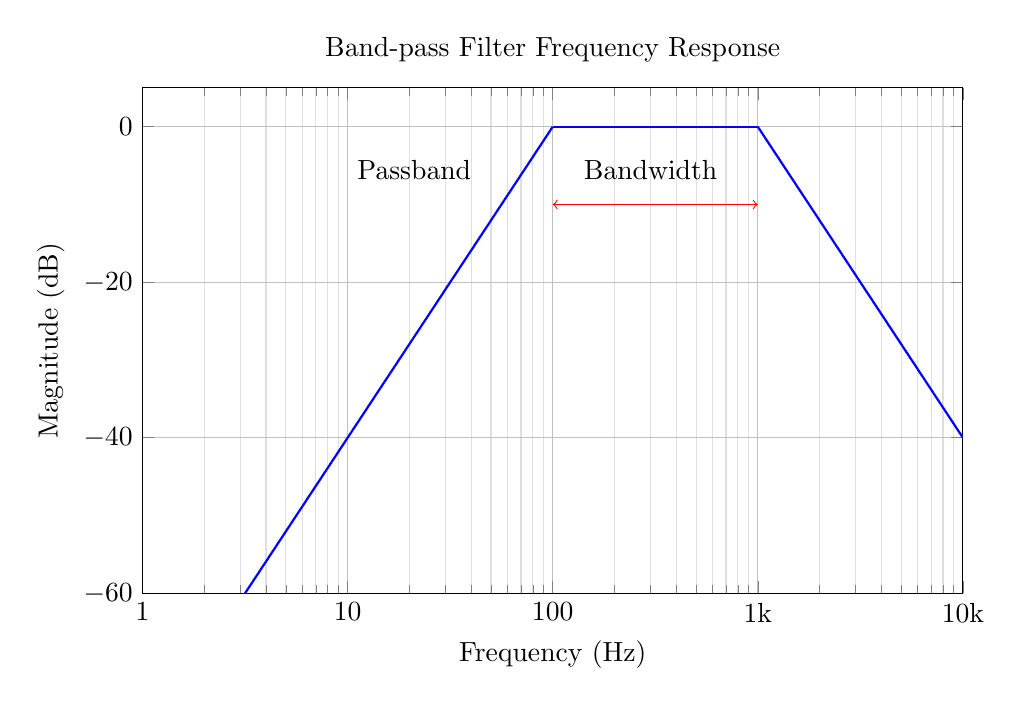
\begin{tikzpicture}
\begin{axis}[
    width=12cm,
    height=8cm,
    xlabel={Frequency (Hz)},
    ylabel={Magnitude (dB)},
    xmode=log,
    xmin=1, xmax=10000,
    ymin=-60, ymax=5,
    xtick={1,10,100,1000,10000},
    xticklabels={1,10,100,1k,10k},
    ytick={-60,-40,-20,0},
    grid=both,
    minor grid style={gray!25},
    major grid style={gray!50},
    title={Band-pass Filter Frequency Response},
]

% Low-frequency rolloff
\addplot[domain=1:100,samples=100,blue,thick] {-40*log10(100/x)};

% Passband
\addplot[domain=100:1000,samples=100,blue,thick] {0};

% High-frequency rolloff
\addplot[domain=1000:10000,samples=100,blue,thick] {-40*log10(x/1000)};

% Annotations
\node[anchor=north west] at (axis cs:10,-3) {Passband};
\draw[<->,red] (axis cs:100,-10) -- (axis cs:1000,-10);
\node[anchor=south] at (axis cs:300,-8) {Bandwidth};

\end{axis}
\end{tikzpicture}
\caption{Ideal Bandpass Filter Response}
\end{figure}


\subsection{Tukey Window}
\label{dsp:tukey}

Window functions are function often used in \acrshort{dsp} and are zero-valued outside of an interval. The Tukey window, also known as the \textit{cosine-tapered window} is one of the more popular window methods, and its mathematical function is described as such: 

\[
    w(x)= 
\begin{cases}
    \frac{1 + \cos{2 \pi \alpha (x + \frac{1-\alpha}{2})}}{2}, & \text{if } x \leq \frac{1-\alpha}{2}\\
    1,              & \text{if } \frac{\alpha}{2} < x \leq \frac{\alpha}{2}\\
    \frac{1 + \cos{2 \pi \alpha (x - \frac{1-\alpha}{2})}}{2}, & \text{if } x > \frac{1-\alpha}{2}
\end{cases}
\]

This window becomes a rectangle when $\alpha = 0$.


\subsection{Resampling}

Also known as sampling-frequency conversion, resampling is the act of modifying the sampling rate of a discrete signal to obtain a new discrete representation of this data. For signal data, lots of samples are usually recorded, but the amount needed to perform calculations or observe patterns does not require this much data. Thus, one can downsample the data to decrease memory usage for storage, as well as time for processing this data. \\


\subsection{Butterworth}

TBI.
\section{Deep Learning}

% Deep Learning
\acrfull{dl} is a subset of \acrshort{ml} and \acrshort{ai}, where the objective is to learn underlying representations of data \cite{lecun2015deep}. In \acrshort{dnn}s, neurons act as the fundamental building blocks. Layers of neurons are grouped into three categories of layers: input-, output- and \textit{hidden layers}.  

\begin{figure}[!h]
    \centering
    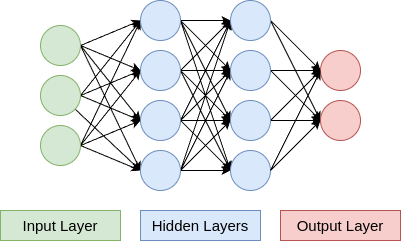
\includegraphics[width=0.5\linewidth]{figures/dnn.png}
    \caption{Example of a dense neural network with one input layer, two hidden layers and one output layer}
    \label{fig:densenn}
\end{figure}

We mainly differentiate between three subcategories of \acrshort{dl}:

\begin{itemize}
    \item \textit{Supervised learning}: Data is labeled, and the goal of the network is trained to make sure the outputs match these labels.
    \item \textit{Unsupervised learning}: The network learns patterns exclusively from unlabeled data and tries to learn the underlying structure of the input vectors \cite{KARHUNEN2015125}. 
    \item \textit{Semi-supervised learning}: Some data may be labeled
\end{itemize}



\subsection{Fully Connected Neural Networks}
\label{back:linear}

\acrfull{fcnn} are fundamental networks used in many \acrshort{dl} models. Also called dense or linear networks, they are characterized by all neurons being connected between two layers (see Figure \ref{fig:densenn}). 

In the forward pass, linear layers transform the input data, mapping an input vector to an output vector using learnable parameters. The operation can be defined as follows:
\begin{equation}\label{f:wxb}
    \mathbf{y} = \mathbf{w}x+b
\end{equation}
Here, $x$ is the input vector, \textbf{$w$} is the weight matrix, $b$ is the bias, and \textbf{$y$} is the output vector.

\begin{figure}[!h]
    \centering
    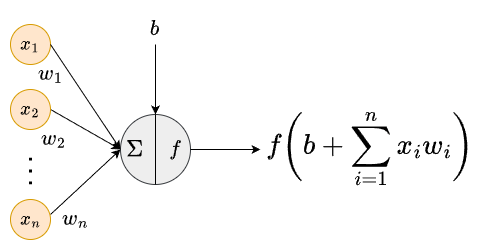
\includegraphics[width=0.7\linewidth]{figures/dl.png}
    \caption{Neurons $x$ in a layer with their weights $w$, a bias $b$ and an activation function $f$}
    \label{fig:dl}
\end{figure}

Furthermore, an activation function $f$ is applied to the output to achieve \textit{nonlinearity}. By applying $f$ to the output $y$, we now get the equation:
\begin{equation}\label{f:fwxb}
    \mathbf{z} = f(\mathbf{y}) = f(\mathbf{w}x+b)
\end{equation}

Some of the more popular activation functions include \cite{szandala2021review}: 

\begin{equation}
    Relu(z) = max(0, z)
\end{equation}

Relu (Rectified Linear Unit) was stated to be the most popular activation function as late as 2018. Its forward and backward pass steps quickly, thus enabling more efficient training compared to other alternatives.

\begin{equation}
    \sigma(z) = \frac{1} {1 + e^{-z}}
\end{equation}

The sigmoid activation is very popular because its range is $[0,1]$, compared to other functions, is rather limited and represents a probabilistic value. This makes it good at outputting probabilistic values.

\begin{equation}
    tanh(x) = \frac{e^x - e^{-x}}{e^x + e^{-x}} = \frac{1 - e^{-2x}}{1 + e^{-2x}}
\end{equation}

Like sigmoid, the hyperbolic tangent has outputs in a relatively small range $[-1, 1]$.

After the forward pass is performed, the network will update its weights. This is done by using a \textit{cost}, or \textit{loss} function and using the resulting loss to calculate the networks' gradients before an optimizer, such as \acrfull{sgd} \cite{Rumelhart1986, Bottou2012}, updates the weights before the following forward pass. For unsupervised networks specifically, two of the more commonly used loss functions include: \\

\textbf{\acrfull{mse}}

\begin{equation}\label{eq:mse}
    \mathcal{L}_{\text{MSE}}(x, \hat{x}) = \dfrac{1}{N}  \sum_{i=1}^{N}(x_i-\hat{x}_i)^2
\end{equation}

The \acrshort{mse} loss function is a commonly used loss function. It punishes bigger differences by squaring the difference between two elements in the prior $x$ and the posterior $\hat{x}$. It then outputs the mean of all the squarred errors computed. \\

\textbf{\acrfull{mae}}

\begin{equation}\label{eq:mae}
    \mathcal{L}_{\text{MAE}}(x, \hat{x}) = \dfrac{1}{N}  \sum_{i=1}^{N}|x_i-\hat{x}_i|
\end{equation}

The \acrshort{mae} loss function is similar to the \acrshort{mse} function. The difference is that the \acrshort{mae} function returns the absolute value of the distance between two distributions $x$ and $\hat{x}$, thus equally punishing all errors. \\

The major bottleneck of all kinds of machine learning techniques is data. The more diverse and varied a . \\

Linear layers have several advantages, such as computational efficiency, flexibility as well as intrerprebility, where the weight and bias vectors can be interpreted as learned parameters. They also serve as building blocks for other components, such as \acrshort{rnn}s \cite{schmidt2019recurrent}, \acrshort{lstm}s \cite{lstm} or even more novel architectures such as the transformer\cite{vaswani2017attention}. \\ 

However, linear layers have several limitations. Due to their inherent linearity, they are prone to \textit{overfitting} and struggle to capture complex relationships in data. This can limit their ability to extract more complex features, potentially reducing some of the model's discriminative power. Furthermore, the size of linear layers can become problematic, especially in \acrshort{fcnn}s. Each neuron connection between layers requires storing weights and biases, which increases the overall model size. For a smaller dense network where the layers are of size $[10, 5, 1]$, the total amount of parameters becomes:
$$\begin{aligned}
S &= (10 \times 5 + 5) + (5 \times 1 + 1) \
&= 50 + 5 + 5 + 1 \
&= 61 \text{ parameters}
\end{aligned}$$
Assuming each parameter is stored as a single-precision floating-point number (\texttt{Float32}, 4 bytes), the total memory size is:
$$\begin{aligned}
\text{Memory size} &= 61 \text{ parameters} \times 4 \text{ bytes/parameter} \
&= 244 \text{ bytes}
\end{aligned}$$ While 244 bytes is small, larger dense networks can quickly consume gigabytes of memory. This can create bottlenecks for hardware accelerators like \acrshort{gpu}s, which typically have less VRAM compared to the \acrshort{ram} available to \acrshort{cpu}s.
\subsection{CNN - Convolutional Neural Networks}
\label{back:cnn}

\acrfull{cnn} \cite{}, a specialized type of feed-forward neural network, has become a cornerstone in \acrshort{dl} architectures. Building upon simpler structures like the linear layer discussed in section \ref{back:linear}, CNNs introduce a powerful approach to processing matrix data, especially images.
The foundations of CNNs can be traced back to neurobiological research in the 1960s on the visual cortex \cite{hubel1962receptive}, but they were first properly introduced to the \acrshort{ml} field in 1990 by Yan LeCun \cite{NIPS1989_53c3bce6}. Since then, CNNs have undergone significant developments, leading to breakthroughs in various fields of artificial intelligence. \\

\begin{figure}[!h]
    \centering
    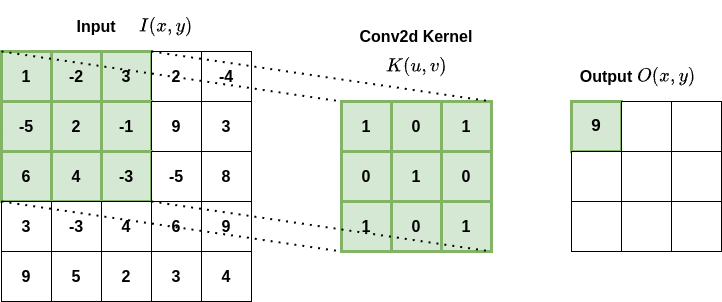
\includegraphics[width=0.8\linewidth]{figures/convolution.png}
    \caption{Example of a 2D Convolutional operation}
    \label{fig:2dconv}
\end{figure}

At their core, CNNs rely on kernel operations, primarily convolutions, to calculate features. The convolution is a mathematically operation which can be defined continuously as following:

\begin{equation}
(f * g)(t) = \int_{-\infty}^{\infty} f(\tau) g(t - \tau) d\tau
\label{eq:contconv}
\end{equation}

and discretely as such:

\begin{equation}
   (f * g)(x, y) = \sum_{m=0}^{M-1} \sum_{n=0}^{N-1} f(m, n)g(x-m, y-n) 
\label{eq:conv}
\end{equation}

Here $f$ is the input matrix, $g$ is the kernel, $m$ and $n$ is the 

The convolutional operation is essentially multiple matrix multiplication between different regions in the data and a kernel. These multiplications can be performed in a parallelized manner. Matrix multiplications have undergone significant improvement over the years CITE, and have with the introduction of CUDA, been further optimized for better suited hardware architectures such as \acrshort{gpu}s. With the rapid improvements of \acrshort{gpu}s, especially by NVIDIA, the computational efficiency of both linear and convolutional layers has improved drastically. This has resulted in overall lower energy requirements for model training, reduced training times and the introduction of distributed large-scale model training \cite{mungoli2023scalable}. \\ 

Unlike fully connected layers that compute global interactions, convolution operations in CNNs focus on local regions data. This localized approach allows for improved feature extraction, making them particularly effective for tasks involving spatial data such as image recognition, object detection, and segmentation. \\


The power of CNNs lies in their ability to automatically learn hierarchical feature representations. Lower layers typically detect simple features like edges or colors, while deeper layers combine these to recognize more complex features. This hierarchical learning, coupled with parameter sharing and local connectivity, enables \acrshort{cnn}s to be both computationally efficient and highly effective at capturing relevant features from high-dimensional data. \\

Due to \acrshort{cnn}s inherent quality of feature extraction, they are not as prone to the vanishing gradient problem \cite{tan2019vanishing} as linear layers. This occurs when gradients propagated backward through the layers become very small, making it difficult for the network to update its weights effectively. \\

Only the size of the kernel is used to stored neurons when performing cross correlation convolution, compared to linear layers where all the weights between layers needs to be stored. \acrshort{cnn}s are highly applicable to numerous different tasks, such as recognition and classification. \\

\subsubsection{Pooling}

Typically, a convolution is followed by an activation function $f$ and then a pooling operation. A pooling operation works like a filter $k$, selecting a certain value from a subset of the input vector based on a heuaristic. The three most common operations are \textit{max pool}, \textit{min pool} and \textit{avg pool}. Out of these, the \textit{max pool} operation operation is most commonly used. This operation reduces dimensionality, outputting only the most important feature for future layers. \\

\begin{figure}[!h]
    \centering
    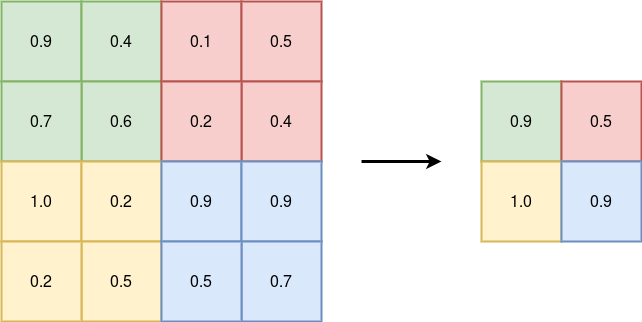
\includegraphics[scale=0.4]{figures/pooling.png}
    \caption{Example of a $2 x 2$ max pool operation with stride 2}
    \label{fig:maxpool}
\end{figure}

In figure \ref{fig:maxpool}, we see an input matrix $M$ where each 2x2 submatrix is being filtered by choosing the maximum element $\hat{M}_{max}$. The filter then strides across $M$ by two elements, repeating the operation until $M$ has been completely filtered.
\clearpage
\subsection{Autoencoder}

Autoencoders are specific types of neural networks used to learn efficient encodings of unlabeled data and then decode them to reconstruct the original data \cite{bank2021autoencoders}. Autoencoders consist of two models, the encoder $E_\phi$ and the decoder $D_\theta$. The relationship between these can be formulated as such: 

\begin{equation}\label{eq:enc}
E_\phi: X \rightarrow Z 
\end{equation}
\begin{equation}\label{eq:dec}
D_\theta: Z \rightarrow X
\end{equation}

$E_\phi$ compresses data $X$ into a latent representation $Z$. $D_\theta$ then decodes $Z$, thus outputting a reconstructed dataset of the same dimensions as the input. $E_\phi$ can be seen as a compressing model, while $D_\theta$ can be seen as a decompressing model. This is further showcased in figure \ref{fig:aediagram}. 

\begin{figure}[!h]
    \centering
    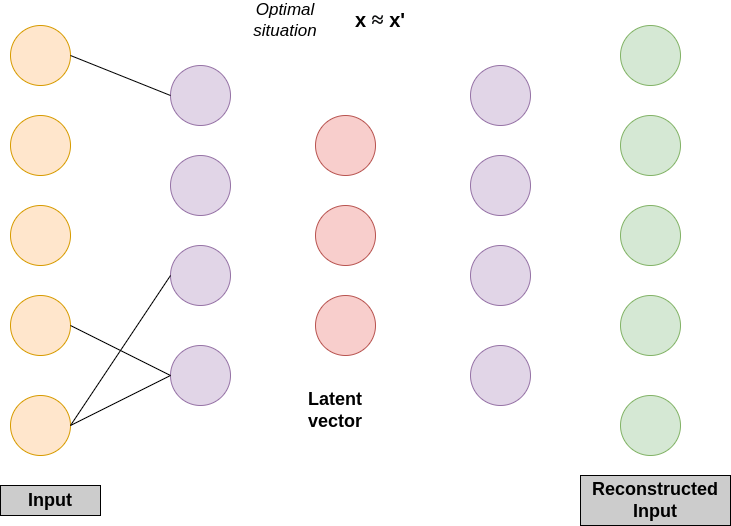
\includegraphics[scale=0.4]{figures/ae.png}
    \caption{Example of a dense autoencoder architecture}
    \label{fig:aediagram}
\end{figure}

The optima for any kind of autoencoder becomes that of lossless encoding, which can be described as such:

\begin{equation}
    X' = D_\theta(E_\phi(X))
\end{equation}

As mentioned in Section \ref{back:linear}, dense networks can struggle with feature extraction. This is also the case for dense autoencoders. By introducing convolutional layers, the autoencoder becomes more adept at image reconstruction and denoising \cite{zhang2018better}. These networks are called convolutional autoencoders (\acrshort{cae}).  \\

When the model is sufficiently trained for a specific task, $D$ \textit{may} become unnecessary for certain applications such as data reconstruction and denoising \cite{vincent2010stacked}. If the primary goal is feature extraction or dimensionality reduction, $E$ alone can be used to map input data to the lower-dimensional latent space. By utilizing only $E$, the overall complexity and size of the model $M$ can be reduced, which may be beneficial in scenarios with computational or memory constraints. For other tasks, such as autoencoders, include image reconstruction \cite{7797236}, signal analysis \cite{andrysiak2016machine}, and anomaly detection \cite{bank2021autoencoders}, the whole model is often needed.
\subsubsection{Latent Space}

The latent space $Z$ in autoencoders aims to capture essential features of the input data $X$ in a lower-dimensional representation. However, traditional autoencoders face limitations in their generative capabilities [CITE]. While they are trained to reconstruct original data accurately, they typically lack the ability to generate new, diverse samples from $Z$.
This limitation arises from the fact that regular autoencoders do not impose any specific structure on $Z$ beyond compressing the $X$. As a result, the latent representations may not be continuous or meaningful for interpolation and generation tasks.



\subsubsection{Loss functions for autoencoders}

The goal of an autoencoder is to make the reconstructed output $\hat{X}$ as close to the input $X$ as possible. Given this, the loss function used for these networks can be seen as a distance metric, where the objective is to minimize the distance $d$ between input and output:

\begin{equation}
    \mathcal{L}(\theta; X) = d(X, \hat{X}) = d(X, f_\theta(X))
\end{equation}
The optimization problem can then be formulated as:
\begin{equation}
    \theta^* = \argmin_{\theta} \mathbb{E}_{X \sim p_{\text{data}}(X)}[\mathcal{L}(\theta; X)]
\end{equation}
where $\theta^*$ are the optimal parameters for the network. Some of the more common loss functions used for autoencoders includes: \\

\clearpage


In addition to the issues with regular autoencoders in regards to decoding the latent space, these autoencoders have several disadvantages, including:

\begin{itemize}
    \item \textbf{Overfitting}: If the encoder and decoder become too powerful, they can learn to simply copy the input data to the output data.
    \item \textbf{Lack of regularization}: This can lead to poor generalization to unseen data
    \item \textbf{Input sensitivity}: Noise in the input data may potentially lead to large changes in the latent space
    \item \textbf{Interpretability}: The latent space may not be interpretable or correspond to meaningful features of the data
    \item \textbf{Encoding determinism}: Regular autoencoders don't account for uncertainty or multiple plausible interpretations of the input.
\end{itemize}
\clearpage
\subsection{Variational Autoencoder}
\label{back:vae}

The \acrfull{vae} \cite{kingma2022autoencodingvariationalbayes} is a type of autoencoder that aims to solve the lack of generative capabilities within regular autoencoders. \acrshort{vae}s are generative models that sample the latent space through a probabilistic distribution. This makes them suitable for image generation tasks \cite{vahdat2020nvae}, something regular autoencoders are unable to do due to their deterministic latent representation.

\begin{figure}[!h]
    \centering
    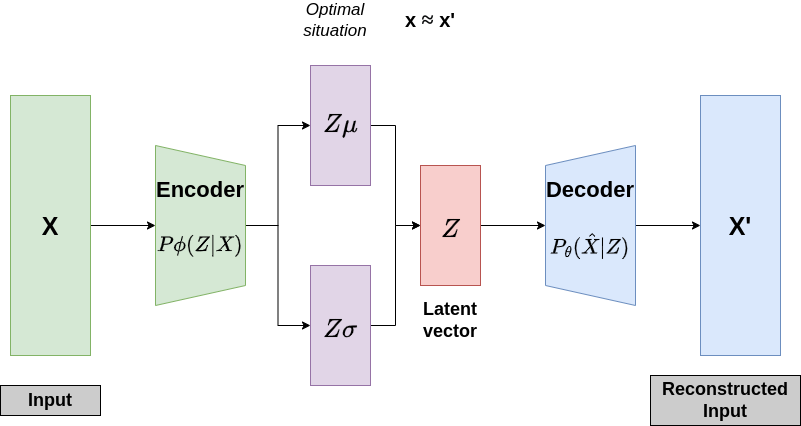
\includegraphics[scale=0.4]{figures/vae.png}
    \caption{Variational Autoencoder Architecture Diagram}
    \label{fig:vaediagram}
\end{figure}


\subsubsection{Reparametrization Trick}
\label{back:reparam}

\acrshort{vae}s can be trained efficiently using backpropagation due to a technique known as the \textit{reparameterization trick} \cite{kingma2022autoencodingvariationalbayes}. This is necessary because \acrshort{vae}s involve sampling from a stochastic latent variable $z$, which would normally hinder gradient-based optimization.

The idea is to express the sampling of $z$ from the approximate posterior $q_\phi(z|x) = \mathcal{N}(\mu, \sigma^2)$ as a deterministic function of the encoder outputs ($\mu$ and $\sigma$) and an additional noise variable $\epsilon$. Specifically:
\begin{equation}
    z = \mu + \sigma \odot \epsilon, \quad \epsilon \sim \mathcal{N}(0, I)
\end{equation}

Here, $\odot$ denotes element-wise multiplication. This formulation allows gradients to flow through the sampling process, enabling end-to-end training of the model.

The reparameterization trick transforms the optimization problem from one involving expectations over $q_\phi(z|x)$ to one involving expectations over $p(\epsilon)$, which is fixed and independent of the model parameters ($\phi$ and $\theta$):

\begin{equation}
    \mathbb{E}_{z \sim q_\phi(z|x)}[f(z)] = \mathbb{E}_{\epsilon \sim \mathcal{N}(0,I)}[f(\mu + \sigma \odot \epsilon)]
\end{equation}

This formulation makes training of \acrshort{vae} models feasable, even for gradient based optimizers, such as \acrshort{adam} or \acrshort{sgd}.




\subsubsection{Evidence Lower Bound}
\label{back:elbo}
In the context of \acrshort{vae}s, \acrshort{elbo} is commonly used as a loss function. \cite{lygerakis2024edvaeentropydecompositionelbo}. It consists of two parts, the reconstruction likelihood $\mathcal{L}_{\text{rec}}$ and the prior constraint $\mathcal{L}_{\text{reg}}$:
\begin{align}
\mathcal{L}_{\text{ELBO}}(\theta, \phi; x) &= \mathcal{L}_{\text{rec}}(\theta, \phi; x) + \mathcal{L}_{\text{reg}}(\phi; x)  
\end{align}
where:
\begin{align}
\mathcal{L}_{\text{rec}}(\theta, \phi; x) &= \mathbb{E}_{q_\phi(z|x)}[\log p_\theta(x|z)] \\
\mathcal{L}_{\text{reg}}(\phi; x) &= -D_{\text{KL}}(q_\phi(z|x) \| p(z))
\end{align}
$\mathcal{L}_{\text{reg}}$ is the negative \acrfull{kld} \cite{10.1214/aoms/1177729694}, which can be further formulated as:
\begin{equation}
    D_{\text{KL}}(q_\phi(z|x) \| p(z)) = \mathbb{E}_{q_\phi(z|x)}\left[\log \frac{q_\phi(z|x)}{p(z)}\right]
\end{equation}
$D_{\text{KL}}$ is always non-negative $(\geq 0)$ and is a statistical method used to quantify the proximity between two probability distributions \cite{shlens2014notes}. 
The reconstruction likelihood $\mathcal{L}_{\text{rec}}$ can be computed in different ways depending on the nature of the input data. For binary data, it is typically computed as a binary cross-entropy loss:
\begin{equation}
\mathcal{L_\text{rec}}(\theta, \phi; x) = - \mathbb{E}_{q_\phi(z|x)}[\mathcal{L}_{\text{BCE}}(x, z)]
\end{equation}
where $\mathcal{L}_{\text{BCE}}(x, z)$ is defined as:
\begin{equation}
\mathcal{L}_{\text{BCE}}(x, z) = \frac{1}{N} \sum_{i=1}^{N} \left( x_i \log p_\theta(x_i|z) + (1 - x_i) \log(1 - p_\theta(x_i|z)) \right)
\end{equation}
For continuous data, more novel adaptations \cite{lygerakis2024edvaeentropydecompositionelbo} often use the \acrshort{mse} loss as shown in equation \ref{eq:mse}, thus giving:
\begin{equation}
    \mathcal{L}_{\text{rec}}(\theta, \phi; x) = \mathbb{E}_{q_\phi(z|x)}[\|x - \hat{x}\|^2]
\end{equation}
where $\hat{x} = p_\theta(x|z)$ is the reconstructed input.
The two losses combined aims at providing a total loss that balances reconstruction quality and the prior regularization \cite{lin2019balancingreconstructionqualityregularisation}.

\subsubsection{Minimizing the ELBO Loss}
The objective in training a \acrshort{vae} is to minimize the negative \acrshort{elbo}, which is equivalent to maximizing the \acrshort{elbo} itself. This optimization problem can be formulated as:

\begin{equation}
    \theta^*, \phi^* = \argmin_{\theta, \phi} \mathbb{E}_{x \sim p_{\text{data}}(x)}[-\mathcal{L}_{\text{ELBO}}(\theta, \phi; x)]
\end{equation}

where $\theta^*$ and $\phi^*$ are the optimal parameters for the decoder and encoder, respectively. By minimizing the negative \acrshort{elbo}, we simultaneously optimize for better reconstruction of the input data (through $\mathcal{L}_{\text{rec}}$) and a latent space distribution that closely matches the prior (through $\mathcal{L}_{\text{reg}}$). This process encourages the \acrshort{vae} to learn a meaningful and structured latent representation of the input data while maintaining the ability to generate new samples \cite{kingma2022autoencodingvariationalbayes}.
\subsection{Data Processing and Mixed Precision Training}
\label{back:data}

\subsubsection{Data Normalization}

Normalization is a technique of which data is transformed from it's original scale, to a more standard scale \cite{ali2014data}. These techniques are normally used when the dataset has elements of different ranges. Normalization can contribute to faster convergence, and it's why they are as commonly used when preprocessing data. 

\textbf{MinMax Normalization} 

This algorithm transforms data to a specified range, most often $[0, 1]$ but it can also be $[-1, 1]$ or any other range.
Minmax normalization can be described as follows:

\begin{equation}
   x_{\text{normalized}} = \dfrac{x - x_{min}}{x_{max}-x_{min}}
\end{equation}
\vspace{0.2cm}

where $x$ denotes the data, $x_{min}$ and $x_{max}$ is the minimum and maximum in $x$. \\

\subsubsection{Half Precision Training}

Working with large datasets and \acrshort{dnn}s can be rather time- and resource consumptive. To address this, one can cast the datatype from single precision to half precision, along with weights, biases and losses. This will reduce loss of accuracy and information, but it can drastically lower memory consumption and decrease training time. It is important to note that casting of data occurs with normalization techniques, the order of which operation happens first is quintessential. If the data is casted to half precision before normalization, the normalization will be based on a slightly inaccurate representation of the data, but the computation of the normalized data will be faster. If normalization were to occur first, less detail about the data would be lost, but at the expense of being more computational intensive. \\

\textbf{Mixed precision training}

Mixed precision training, introduced in 2018 \cite{micikevicius2018mixed}, is a technique where the weights, activations and biases of a neural network is stored in single precision, while the data itself stays in it's original format. It allows for reduced memory consumption, while also speeding up operations of deep neural nets. Additionally, the amount of $\si{\kilo\watt\hour}$ required to train the neural nets would decrease, thus reducing both the cost and the environmental tax by training neural nets. This becomes more important the larger the datasets, models and the sheer amount of GPUS required to train massive workloads. This introduce the concept of loss scaling, where the losses needs to be adjusted based on the weights. \\

\mycomment{
\subsection{Dataloaders}

If the datasets contain information about the data and how to retrieve a single instance, the dataloaders job is to create an object that can be iterated over, containing $n$ amount of batches, and transferring these data to the wanted devices. In the case of data parallel multi-gpu training, when the data is loaded, it's \textit{sharded} across the different gpus, in a manner that balances the load of each gpu. Let's say we have a batch  of size $[4, 5, 5]$ and we have two gpus available. The dataloader can split this Tensor in two batches, where each of the gpus get a tensor of size $[2, 5, 5]$. By sharding the data along the first axis, ideally we can half the amount it takes, not taking data transfer time into consideration. 

\begin{figure}[!h]
    \centering
    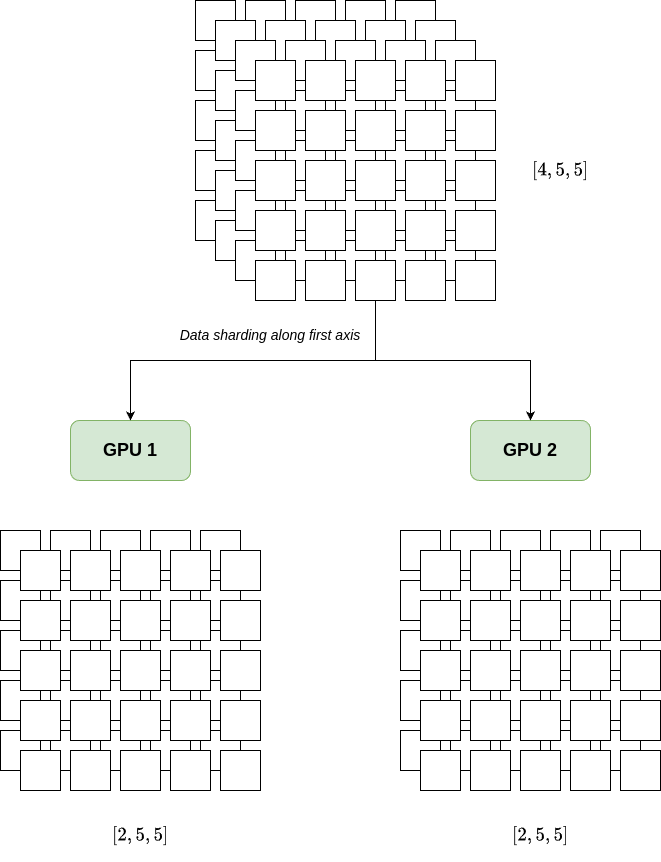
\includegraphics[scale=0.4]{figures/sharding.png}
    \caption{Example of data sharding with 2 gpus, and a original Tensor of size [4,5,5]}
    \label{fig:sharding}
\end{figure}


\textbf{Parallel loading}

When iterating over a dataloader, each element of the batch is retrieved and undergoes transformations. Depending on the batch size and  the size of the data, this procedure can be very resource-intensive and time-consuming. To mitigate this, we can introduce the concept of parallel batch loading. Instead of gathering and transforming the data sequentially, one can leverage available resources to do this operation in a parallel manner. Algorithm \ref{alg:parallel-batch-loading} details how such an operation is conducted.


\begin{algorithm}
\caption{Parallel Batch Data Loading}\label{alg:parallel-batch-loading}
\begin{algorithmic}
\Require BatchIndices, N
\Ensure BatchData, LoadSingleData
\State Initialize empty list BatchData
\State Create ThreadPool with N threads
\For{each Index in BatchIndices}
    \State Submit LoadSingleData(Index) to executor
\EndFor
\For{each completed Future from executor}
    \State Data $\gets$ Future.result()
    \State Append Data to BatchData
\EndFor
\State \Return BatchData
\end{algorithmic}
\end{algorithm}
}

\subsubsection{Overfitting and Early Stopping}

Overfitting is a common problem within \acrlong{ml} \cite{srivastava2014dropout}. It occurs when a model is trained , and fails to fit additional data. In addition to popular techniques such as dropout \cite{srivastava2014dropout}, \textit{early stopping} is a regularization technique that aims to avoid overfitting. When training an optimizer such as \acrshort{adam} \cite{kingma2017adam}, or \acrshort{sgd} \cite{Rumelhart1986, Bottou2012}, one can notice when a model is overfitting by studying the validation loss. If the validation loss $L_v$ starts increasing, the early stop mechanism will stop the training altogether if no improvement of $L_v$ is found after $p$ number of epochs. A formal definition can be given as such:

\begin{align*}
&\text{Stop at epoch } T \text{ if:} \\
&\forall i \in \{T-p+1, ..., T\}: L_v(i) > L_v^* - \epsilon \\
&\text{where } L_v^* = \min_{j=1}^{T} L_v(j) \\
\\
&\text{Given:} \\
&L_v(t) \text{ is the validation loss at epoch } t \\
&p \text{ is the patience (number of epochs to wait)} \\
&\epsilon \text{ is a small threshold for improvement}
\end{align*}

\subsubsection{Parallelism within \acrlong{ml}}

With rapid evolving deep learning architectures, the importance of scalable model training and networks grows larger each year. It is even estimated that these networks grow 1,5x each year \cite{9499913}, making parallelization a vital topic when it comes to \acrlong{ml} to accommodate ever increasing memory needs. Several different hardware accelerators have been created to best accommodate these needs, the most apparent of these are \acrshort{gpu}s. NVIDIA have for several years dominated this market, and their hardware is becoming faster and increasing in memory. \\

By workers, we mainly refer to \acrshort{gpu}s, but this could also be processors or other types of hardware accelerators such as TPUs.


\subsubsection{Model Parallelism}

\acrshort{dl} models need to store a lot of data. Weights and biases tend to take up a lot of memory, thus requiring the need of splitting up a model across several workers. As an example, given a model $M$ of 50 layers, we can split this model in 2 parts by having a worker $A$ manage the first 25 layers, and worker $B$ manage the latter half.
The overhead of transferring data across these workers can become a bottleneck, so this should only be utilized when absolutely necessary.

\subsubsection{Data Parallelism}

Data parallelism refers to partitioning data across multiple workers. Given a dataset $X$, we can split $X$ across the workers and store a copy of the model $M$ on each worker, calculate gradients across them all and update the trainable parameters for $M$. 

\subsubsection{Hybrid Parallelism}

This kind of parallelization combines the two previously mentioned techniques. First, $M$ is split across several workers, and then $X$ is subsequently split across multiple workers. 
\section{Anomaly Detection}
\label{back:anomdet}

\textit{Anomaly detection} is about identifying observations that can be deemed inconsistent with the rest of the dataset \cite{anomaly}. These anomalies can also be referred as outliers, surprises, exceptions, depending on domain. Anomaly detection can be used on all kinds of data, ranging from images to time-series data. There are 3 main types of anomalies, and those are \textit{point anomalies}, \textit{contextual anomalies} and \textit{collective anomalies}.

\begin{figure}[!h]
    \centering
    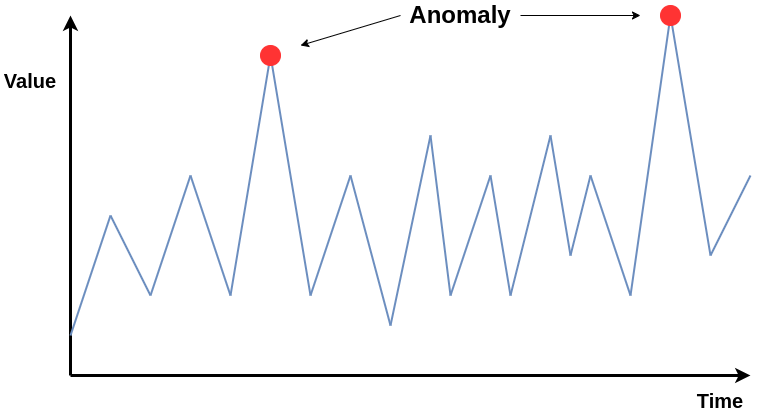
\includegraphics[scale=0.4]{figures/anolay_line.png}
    \caption{Example of anomalies in a time series}
    \label{fig:anomaly_example}
\end{figure}

While point anomalies target single instances that differ from the rest of the dataset, collective anomalies targets groups of instances that together form an anomaly. Contextual ones, as in the word, require context to determine whether or not an anomaly has been detected, and is typically found in time-series data.

Anomaly detection can be performed in a lot of different ways. From common machine learning tasks such as K-means clustering \cite{7507933}, \Gls{svm} \cite{10.1007/978-3-540-28647-9_97}





Given a matrix $a$ of data:

\[
A = \begin{bmatrix}
a_{11} & a_{12} & \cdots & a_{1n} \\
a_{21} & a_{22} & \cdots & a_{2n} \\
\vdots & \vdots & \ddots & \vdots \\
a_{m1} & a_{m2} & \cdots & a_{mn}
\end{bmatrix}
\]

We are interested in finding a region $a_{ij} to a_{kl}$ where $i < k \And j < l$ st. the values within these regions falls outside of the general range


For \acrshort{das} data specifically, anomaly detection can be used for detecting clusters of signals that don't correspond to the predisposed target feature. Registering these outlier signals and receiving real time information about these could prove vital in some cases,  and in best case scenario save lives. 

Dealing with sensitive data 

\subsection{Time series based anomaly detection}

Time series in one dimension is often a great candidate for anomaly detection. Stock market prediction, climate changes and several other series can be used to train networks to recognize point wise anomalies. Layers such as LSTM, RNN and GRU are constructed to store and retrieve information at a later time, thus introducing a memory mechanism. 

\subsection{Image based anomaly detection}

Anomaly detection can also be applied to images. Given a dataset of images with sheep, a image based anomaly detection model would be able to recognize any drastic changes between images. Without the temporal aspect of these problems, convolutional or linear layers are more often used. 

\begin{figure}[!h]
    \centering
    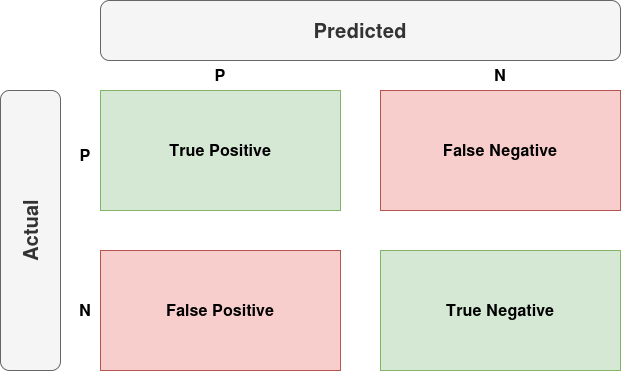
\includegraphics[width=0.5\linewidth]{figures/confmat.png}
    \caption{Caption}
    \label{fig:confmat}
\end{figure}

\section{Related Work}
\label{relwork:anomaly}


\subsection{\acrshort{das} file loading and processing}

One of the file formats used for storing \acrshort{das} data is \acrshort{hdf5}. Many of the implemented libraries for \acrshort{hdf5} files now allow for parallel loading of these files. Biddiscombe (et. al 2012) replaced the IO layer within a \acrshort{hdf5} library ''to allow for parallel loading between simulation and analysis'' \cite{biddiscombe2012parallel}. In later years, \texttt{HDF5.jl}, the HDF5 library in Julia, allows for parallel loading of files, utilizing the message-passing interface (MPI). This can potentially reduce \acrshort{das} file loading times. \\ 

An important aspect of \acrshort{das} processing revolves around frequency analysis, denoising, and other types of filtering. 2D \acrfull{fft}s within 2D linear band pass filtering, and one-dimensional adaptive filtering using \acrfull{fir} filters have all been studied and \cite{daspreproc}. In our preliminary studies, we conducted a performance comparison between Julia and Python for computing 2D Fast Fourier Transforms (FFTs) on \acrshort{das} data using \acrshort{gpu}s. Our results demonstrated that Julia significantly outperformed Python in this specific operation \cite{projthesis}. \\

Public \acrshort{das} datasets are often scarce and hard to find. PubDAS \cite{spica2023pubdas} is a public distribution of several \acrshort{das} datasets worldwide, stored in multiple file formats. Many of these datasets contain scripts containing preprocessing algorithms or visualization code. These techniques are sequential, preprocessing file by file and possibly removing erroneous files. These scripts are mainly single-file Python or MatLab scripts. \\ 

One key aspect of \acrshort{ann}s is the necessity of larger train datasets. Data augmentation techniques such as cropping, resizing, or color grading can increase the available datasets for more vision-based tasks. Another way to increase the total amount of train data is by leveraging \acrshort{gan}s. After training a \acrshort{gan} model, the generator can produce data similar to already collected data. This has yielded great results on \acrshort{das} data \cite{Shiloh:19}, and can be a great way to provide more train data, which in turn can help models detect anomalies more accurately by being trained on a wider variety of data. \\

\subsection{Anomaly detection algorithms for \acrshort{das} data analysis}

The most commonly used algorithms regarding machine learning have traditionally been centered around Kmeans clustering, K nearest neighbors, and  Support Vector machines \cite{10.14778/3538598.3538602, 10.1145/3444690}. These have proven to be efficient, especially when dealing with unlabeled data. These clustering techniques are good at outlining groups grouping them, and finding outliers while dealing with them. One article found k means to be a great choice when dealing with traffic analysis and detection \cite{7507933}. Others have looked at svms as another solid option when dealing with anomaly detection \cite{10.1007/978-3-540-28647-9_97}. Omar (et al 2013) \cite{omar2013machine} looked in general at machine learning techniques such as SVMs, k means, decision trees and bayesian networks, and found that supervised ones generally outperforms their unsupervised counterparts when the types of anomalies where known beforehand, but struggle with novel anomalies. \\ 

Alongside well-known clustering techniques such as k means and knn, \acrfull{dbscan}, first published in 1996 \cite{10.5555/3001460.3001507} is a well-known clustering technique suited for outlier detection in multidimensional datasets. It's still being researched and improved as of this date for multivariate time series \cite{waltz2024time}, and has numerous implementations in different frameworks and languages.  


%%%%%%%%%%%%%%%%%%%%%%%%%%%%
%% AE DAS $$$$$ 
%%%%%%%%%%%%%%%%%%%%%%%%%%%%%%%%%%%%%%%%%%%%
An effort has been made into trying to improve autoencoders for anomaly detection \cite{tan2023improving}

Vae for time series \cite{desai2021timevae}


Ball2017 - dl in remote sensing

apSensingo2019railwaydas - powerpoint
s21196627 - dnn microseismic , das
sensors - mdpi ???

In general, autoencoders with linear, convolutional, or recurrent layers, clustering algorithms, and more traditional \acrshort{ml} methods have seen many use-cases within \acrshort{das} research. However, in later years with the later additions of both attention layers, or even \acrshort{gan}s \cite{goodfellow2014generative, goodfellow2016nips}, more novel approaches are being researched. By introducing channel attention and spatial attention to \acrshort{cnn}, one article \cite{eage:/content/journals/10.1111/1365-2478.13355} finds good results for denoising \acrshort{das} signals. 


Label-free autoencoder-based anomaly detection on \acrshort{das} data has been conducted as late as in 2023 \cite{xie2023label}. A combination of a convolutional autoencoder trained on normal-range \acrshort{das} data and a clustering algorithm to locate the feature center was found to beat state-of-the-art supervised networks. Another interesting aspect of this research is the emphasis on model size, creating a sufficient \acrshort{cae} model with only \qty{1.34}{\si{\kilo}} parameters. This research, in particular, has led the ground for our research and the creation of a program for training and comparing several types of autoencoders. \\





\subsection{Other Models}

Zhu (et al. 2023) use ''a pre-trained PhaseNet to generate noisy labels of P/S arrivals in \acrshort{das} data'' and ''applied the GaMMa method to refine noisy labels and build training datasets'' \cite{zhu2023seismic}. A \acrshort{dl} model was then made to detect earthquakes. \\


\acrshort{gan} is another type of generative nn, first proposed by Iain Goodfellow around 2016 \cite{goodfellow2016nips}. These networks have been utilized in models for specifically designed for anomaly detection. A \acrshort{lstm} \acrshort{vae} \acrshort{gan} model was built to detect anomalies within time series \cite{s20133738}. A modification of \acrshort{lstm} \acrshort{gan}, with the inclusion of the attention mechanism \cite{vaswani2017attention}, was built for time-series anomaly detection \cite{bashar2023algan}.ALGAN-DA?
AEGAN-AD \cite{jiang2023unsupervised} uses a \acrshort{gan} based approach to detect anomalies within audio.

Researchers at NTNU constructed a \acrshort{lstm} \acrshort{vae} model for fault detection on a multi-sensor system for maritime systems \cite{9514856} with good success. Deep \acrshort{lstm}-based autoencoders have also been found to be able to detect anomalies within multivariate time-series forecasting problems \cite{alaaDeepLstm2019}.

One issue of concern is online long-distance distributed monitoring applications. By using a combination of a ResNET with a convolutional block attention module (CBAM), one paper is able to achieve real-time inference time cost as low as 3.3ms per sample \cite{photonics9100677}, while still averaging a high accuracy, even for multi-scenario scenes. 


% Huang (et al. 2021) \cite{huang2021esad} semisupervised learning  kl


Anomaly detection, sometimes referred to as outlier detection, is highly relevant within \acrshort{das} research. In 2017, several classical \acrshort{ml} techniques such as Gaussian Mixture Model (GMM), Hidden Markov Model (HMM), Naive Bayes (NB), and Restricted Boltzmann Machine (RBM) were compared to discriminative models, including \acrshort{ann}s \cite{app7080841}. Variations of isolation forests are shown to be able to perform fault detection for mining conveyors\cite{WIJAYA2022110330}. \\

As previously mentioned in chapter \ref{chap:introduction}, label-free anomaly detection has the advantage of requiring a lot less manual labor and can be adapted to multiple datasets. A model that requires only normal-state data, utilizing both autoencoders and the K-means clustering technique, has yielded great results, even beating supervised methods \cite{s23084094}. \\ 

a, \cite{10.14778/3538598.3538602} \cite{10.1145/3444690}.

All this research shows how processing and anomaly detection on \acrshort{das} data is highly relevant. However, most of them do not necessarily concern themselves with available computational power, overall memory consumption, or how to optimize these algorithms for real-time environments, where accuracy, fault tolerance, and inference speed are of utmost importance.



THIS ONE IS HIGHLY RELEVANT AND HAS MANY METRICS \cite{s23021009}

\chapter{Design and Implementation}
\label{chap:method}

This third chapter details the development process of Judas and TinyDAS. We discuss implementation specifics, software selection rationale, and how these programs are designed to contribute to both our research and that of the wider scientific community, in particular members at \acrshort{cgf}.


% JUDAS
\section{Overview}

Judas and TinyDAS are designed to process \acrshort{das} data as efficiently as possible and subsequently detect anomalies within said data. Figure \ref{fig:judasnet_overview} highlights how Judas and TinyDAS can be utilized to both process and train or analyse DAS data.

\begin{figure}[!h]
    \centering
    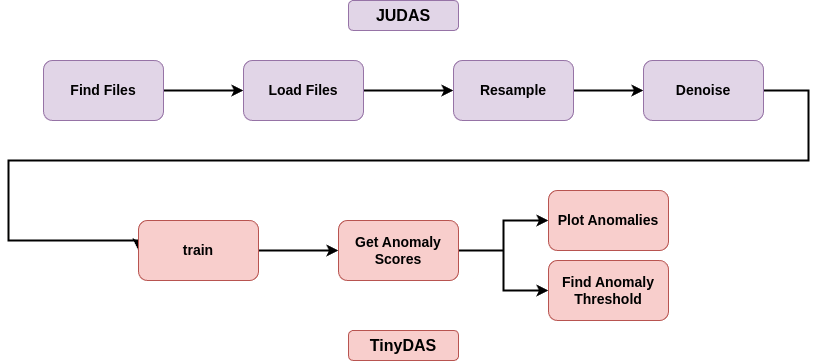
\includegraphics[scale=.4]{figures/api_overview.png}
    \caption{Judas and TinyDAS combined methodflow}
    \label{fig:judasnet_overview}
\end{figure}
\section{Judas}
\label{met:Judas}

Judas, formerly known as Emerald \cite{projthesis}, is a Julia package we've created for internal use for members at \acrshort{cgf}. Our work started last fall, when we saw a limitation of current applications at \acrshort{cgf} for loading \acrshort{das} data from local servers into programs to be able to process and further analyze these data. We chose to write this package in Julia both due to its high performance, and members' familiarity with similar languages such as MatLab and Python. With Julia, we could draw strengths from its ecosystem and build systems to create an easy-to-use library for members to familiarize themselves with. We did so by starting off with a simple python program, that read multiple \acrshort{hdf5} files storing \acrshort{das} data into dataframes. From here, we parallellized certain parts of the code, and opted to store processed data in memory mapped files instead of loading large matrices into memory. This allowed us to work with more data at the same time, as well as decreasing the overall wall time and memory consumption.  

In this section, we will be looking at what changes has been made ever since, from improvements of existent code, to new methods added and the availability of the library for members at \acrshort{cgf}. \\

\subsection{Overview}

Our product is split into two apis. Those being \texttt{Judas} and \texttt{JudasNET}. Judas is the direct continuation from \cite{projthesis}
The \acrshort{api} that's being created is called \texttt{Judas} (Julia and DAS) and is split in 3 modules as well as a seperate Utils file as shown in \ref{fig:ccuda}

\begin{figure}[!h]
    \centering
    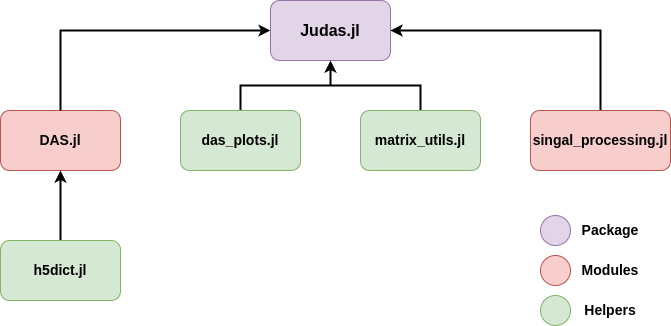
\includegraphics[scale=.6]{figures/judas_overview.png}
    \caption{Overview over our package Judas}
    \label{fig:judasoverview}
\end{figure}


\subsection{Dataset}

Following our previous work, we will be working with data recorded from BANENOR, specifically a train route between Trondheim and Storen with recorded values from the 31st of August 2021 \footnote{Working with national infrastructure requires security clearance, see \ref{app:conf} for more details}. 

\begin{table}[!htbp]
    \centering
    \small
    \begin{tabular}{@{}p{0.3\textwidth}p{0.4\textwidth}p{0.2\textwidth}@{}}
        \toprule
        \textbf{Parameter} & \textbf{Value} & \textbf{Unit} \\
        \midrule
        Experiment & 210830\_NTNU\_Bane\_NOR\_GL8De4F2000 & \\
        File timestamp & 2021-08-31 10:00:01 & \\
        Type of data & Phase rate per distance & rad/m/s \\
        Sampling frequency & 2000.0 & \si{\hertz} \\
        Channel distance & 4.0852 & \si{\meter} \\
        \midrule
        Data shape & 20000 samples \(\times\) 12500 channels & \\
        \midrule
        Gauge length & 8.170401526197452 & \si{\meter} \\
        Sensitivities & 9.362208901094029e6 & r \\
        Regions of interest (ROI) & 1:4:49996 & \\
        \bottomrule
    \end{tabular}
    \caption{BANENOR Experiment Data Summary}
    \label{tab:experiment_data}
\end{table}

As we can see in table \ref{tab:experiment_data}, the total distance of this dataset is approximately 50km, where we have stored data for every 4th sensor across the route. Each file contains 10 seconds of data, leading us to get a matrix of size $20000 x 12500$, where each element is of type \texttt{Float32}, giving us a total of 8GB to be stored for every 10 seconds. This obviously is challenging to work with, so we will go further in depth on how we use resampling and channel decimation to be able to reduce memory usage yet still retain the most important aspects of our signal data. \\


To best showcase what changes and improvements have been made, \ref{fig:apiflow} visualizes the order of high level operations to done on our data. In addition, we will be demonstrating mostly the new additions to the code, as well as the changes to the loading and preprocessing of the data. \\

\begin{figure}[!h]
    \centering
    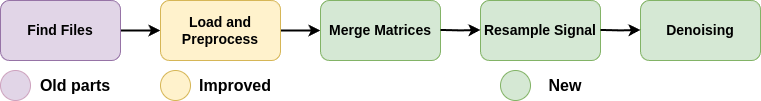
\includegraphics[scale=0.5]{figures/dataflow.png}
    \caption{Dataflow from we read HDF5 files to we are ready to train}
    \label{fig:apiflow}
\end{figure}

\subsection{Pre processing functions}

\subsubsection{Loading \acrshort{das} data}

The \acrshort{das} folder structure has remained largely unchanged. The primary modification involves our data storage approach. Previously, we wrote matrix data to a single large binary file. Now, this data is distributed across multiple files, which are only accessed when specific information is required. This new method optimizes data retrieval and storage efficiency.

Contrary to what was mentioned before, the output of the function \texttt{load\_DAS\_files} has actually changed. Previously, we stored a whole vector of the timestamps for each sample. Not only was this cistly, but actaully totally redundant. If the timestamp of the first row is known, the sampling rate $T$ and which row to look at, one can instead calculate the timestamp like this: 
\lstinline|start_time + MilliSecond(idx * T * 1000)|. This in-place calculation can be done multiple times effectively in Julia using the broadcast operator (.). This ensures that we don't lose essential information before running our data through through the autoencoder

\begin{figure}[!h]
\centering
\begin{subfigure}{.45\textwidth}
  \centering
  \lstinputlisting[language=Julia]{code/dasstructold.jl}
  \caption{Old DAS Struct}
  \label{fig:olddasstc}
\end{subfigure}%
\hfill
\begin{subfigure}{.45\textwidth}
  \centering
  \lstinputlisting[language=Julia]{code/dasstruct.jl}
  \caption{New Layout for DAS struct}
  \label{fig:newdasstc}
\end{subfigure}
\caption{Comparison between different versions of the DAS struct}
\label{fig:dasstccmp}
\end{figure}

From our work on \texttt{Emerald.jl}, the \texttt{find\_DAS\_files} can not be improved much further. 

\lstinputlisting[caption=Parallel processing of \acrshort{das} signal matrices, language=Julia]{code/load_das_files.jl}

\subsubsection{Parallel Resampling}

One of the ways we're able to reduce memory consumption of our program is to resample the signal matrix. What we want to do, is to resample by each sensor, and then combining the results into a new resampled matrix. As we've seen, the original frequency is $2000Hz$, but we want to resample down to $100Hz$, thus only storing $5\%$ of the original data. The following code below shows the implementation of our \texttt{parallel\_resample} function. \\

\lstinputlisting[caption=Implementation of parallel resampling, language=Julia]{code/parallel_resample.jl}

Our parallel resampling approach optimizes performance through memory management and parallel processing techniques. The algorithm proceeds as follows:

\begin{enumerate}
    \item \textbf{Memory Preallocation}: We begin by preallocationg the resultant matrix. This is crucial for performance, as it avoids dynamic memory allocations during the resampling process.
    \item \textbf{Parallel Processing}: We utilize the \texttt{pmap} function from the \texttt{Distributed.jl} package to distribute the resampling workload across multiple processes. Each process is assigned a subset of columns from the input data, allowing for parallel resampling of multiple channels.
    \item \textbf{Resampling}: Within each process, we apply the \texttt{resample} function (from \texttt{DSP.jl}) to individual colums, resampling each channel independently.
    \item \textbf{Data Collection}: To gather the results from the processes, we employ an optimized loop structure. The \texttt{@inbounds} macro disables bounds checking, eliminatin the overhead of boundary checks during array checks. The \texttt{@simd} macro is applied to hint to the compiler to allow for loop reordering, potentially enabling vectorization.
\end{enumerate}


\begin{enumerate}
    \item Judas now make use of multiple processors contra multithreading, seeing major speedups.
    \item Function \texttt{load\_DAS\_files} now writes processed data to a single file back.
\end{enumerate}



\subsubsection{Denoising \acrshort{das} signals}

\lstinputlisting[caption=Denoise function, language=Julia]{code/denoise.jl}

The last addition to \texttt{Judas.jl} is the \texttt{denoise} function. It combines tapering and digital filtering techniques, resulting in an efficient algorithm for \acrshort{das} signal denoising. The function proceeds as follows:

\begin{enumerate}
    \item \textbf{Input validation}: \texttt{denoise} is only performed if tapering is enabled and we are certain the input data is a matrix.
    \item \textbf{Tapering}: A Tukey window (tapered cosine) is applied to mitigate edge effects. Subsequentually, we broadcast the taper across all channels simultaneously.
    \item \textbf{Cutoff Frequency Normalization}: Following, we   normalize the cutoff frequecies by the Nyquist ferquency
    \item \textbf{Digital Filtering}: We utilize the  \texttt{filtfilt} function to apply a zero-phase digital filter, which preserves the phase of the original signal. The filter type provided can be either a lowpass, highpass or a bandpass filter, allowing for selecting approriate filtertype for the scenario. The Butterworth filter design offers a maximally flat frequency response in the passband, providing optimal reduction of noise.
\end{enumerate}

\subsection{General Usage and Distribution}

Our main goal with \texttt{Judas.jl} has been to provide a high performance and easy-to-use library for members at \acrshort{cgf}. To illustrate the ease of use, the following code showcases its simplicity and how users easily can use it alongside other packages. \\

\lstinputlisting[caption=Simple example of how to use Judas, language=Julia]{code/judas_usage.jl}

In addition to the methods we've described in detail, there exist multiple helper methods for plotting and reading/writing \acrshort{das} data. \texttt{Judas.jl} v1.1.0 is currently available for use for members at \acrshort{cgf}. 

\subsection{Evaluation}

In order to evaluate the improvements and additions to this package, we will be performing benchmarks both on individual functions, as well as the overall runtime of a simple usecase. Hereby is a list of different experiments to be conducted:

\begin{itemize}
    \item \textbf{Experiment 1}: Parallel Resample function
    \item \textbf{Experiment 2}: Loading and Processing \acrshort{das} data
\end{itemize}

% \section{Programming Languages and Frameworks}

Our initial decision was to continue using Julia for our \acrshort{dl} methods, and train our models on the same dataset provided by \acrshort{cgf}. We created a Julia package called JudasNET, containing code for training different \acrshort{ai} models. However, due to severe computational limitations, we were unable to continue our work on the previous decision. With only 11GB of VRAM, the single \acrshort{gpu} available quickly became a bottleneck. Not only do we need to store batches of \acrshort{das} data matrices, but we also need to store the weights and biases of our models. By switching to a open source dataset, we would be able to use \Gls{idun}, and leverage multiple \acrshort{gpu}s and in general more computational power. Since the BANENOR dataset is close sourced, we would not be able to train our models on any other resources outside of those provided by \acrshort{cgf}.

Not only were our attempts at training models unsuccessful, Julia's main framework for \acrshort{ml} training \texttt{Flux.jl} does not provide built in tools for multigpu training. \\  

The more obvious choice would now be to use the Python package \texttt{Pytorch}, which is well established, documented and supports not only data parallel training \footnote{  \href{https://pytorch.org/docs/stable/generated/torch.nn.DataParallel.html}{https://pytorch.org/docs/stable/generated/torch.nn.DataParallel.html}}, but also distributed data parallel training \footnote{\href{https://pytorch.org/tutorials/intermediate/ddp_tutorial.html}{https://pytorch.org/tutorials/intermediate/ddp\_tutorial.html}}. What needs to be mentrioned is that Pytorch is heavily optimized for CUDA and NVIDIA \acrshort{gpu}s, and in general performs significantly better on these accelerators, compared to other alternatives such as AMD, NV, METAL and so on. \\ 

We want to create models where we don't need to change much of our code to run on different accelerators. We also want \acrshort{cgf} to  quickly be able to both continue training and running their own models. NVIDIA \acrshort{gpu}s are generally expensive, many of them reaching prices of tens of thousands of dollars per \acrshort{gpu}. We realize that this would not be feasible for \acrshort{cgf} to invest in right now, and thus we decided to look for other frameworks which supports a broader range of hardware accelerators. \\ 

Due to these constraints, we believe Tinygrad \cite{tinygrad} will be a well suited framework for our usecase.

\subsection{TinyGrad}











\mycomment{



DOI \cite{doi:10.1137/141000671}

\subsection{Flux.jl}
\label{back:flux}

Flux is a machine learning library written entirely in Julia released and published in 2018 \cite{Flux.jl-2018, Innes2018}. It allows the user to write their own machine-learning libraries. \acrshort{gpu} support is also native, through the inclusion of \texttt{CUDA.jl} \cite{Besard_2019}. We will be writing all of our models using Flux, or \texttt{Zygote.jl}, which \texttt{Flux.jl} is based on. 

Although \texttt{Flux.jl} is the preferred way to work with \acrshort{ai} in Julia, other prominent alternatives exists as well. \texttt{MLJ.jl} \cite{blaom2020flexible} \cite{Blaom2020} is a framework provided by the Alan Turing Institute\texttrademark, providing interfaces and functions for working with about 200 machine learning models. 

\texttt{Tensorflow.jl} is a Julia package which wraps Tensorflow functions from Python to be able to work with ethem

Julia has support for working on outlier detection as follows: \cite{muhr2022outlierdetectionjl}.

A list of all packages used in addition to Flux.jl can be found in the appendix \ref{app:packages}.

}

\section{TinyDAS}

TinyDAS is a program we've created to easily be able to train, and test different types of autoencoder models for anomaly detection. The main ideas behind creating this program are as follows:

\begin{enumerate}
    \item New autoencoder models are easy to add
    \item Easy to tune configurations
    \item Scalable from single core computer to distributed systems.
    \item The program is not tied to any particular hardware accelerator architecture
    \item Support for half precision training
    \item Support for transfer learning and early stopping
    \item Testing of autoencoders should be easy to add
\end{enumerate}

Based on these conditions, our choice of framework was tinygrad \ref{back:tinygrad}, mainly since the framework is designed to be accelerator-independent.

\subsection{\acrshort{api} design}

\subsubsection{Early Stopping}

Even though the model loss ideally should decrease to eventually reach zero almost immediately, this is never the case. Overfitting is when the loss starts increasing, never to return to its best value. To avoid spending time and resources on unnecessary training, we implement a useful mechanism called early stopping, which is described as follows:

\begin{align*}
&\text{Stop at epoch } T \text{ if:} \\
&\forall i \in \{T-p+1, ..., T\}: L_v(i) > L_v^* - \epsilon \\
&\text{where } L_v^* = \min_{j=1}^{T} L_v(j) \\
\\
&\text{Given:} \\
&L_v(t) \text{ is the validation loss at epoch } t \\
&p \text{ is the patience (number of epochs to wait)} \\
&\epsilon \text{ is a small threshold for improvement}
\end{align*}


\chapter{Experiments}
\label{chap:exp}

The fourth chapter presents our experiments and is split into two parts: one for \acrshort{das} processing and one for anomaly detection using autoencoders. Both follow a consistent structure: we begin with a detailed description of the dataset, followed by an explanation of the research methodologies. We then justify our choice of evaluation metrics and outline the experimental setups.

\section{Experiment 1: BANENOR}


\subsection{Dataset}


Our first experiment revolves around a \acrshort{das} dataset on a a train route between Trondheim and Storen, and is owned by BANENOR. The dataset spans the entirety of the 31st of August 2021\footnote{Working with national infrastructure requires security clearance, see \ref{app:conf} for more details}. The full route between Trondheim and Storen can be seen in appendix \ref{app:judas}. All the data is stored in hdf5 files.

\begin{table}[!htbp]
    \centering
    \small
    \begin{tabular}{@{}p{0.3\textwidth}p{0.4\textwidth}@{}}
        \toprule
        \textbf{Parameter} & \textbf{Value} \\
        \midrule
        Experiment & 210830\_NTNU\_Bane\_NOR\_GL8De4F2000  \\
        File timestamp & 2021-08-31 10:00:01  \\
        Type of data & Phase rate per distance (rad/m/s) \\
        Sampling frequency & \qty{2000}{\si{\hertz}} \\
        Window duration & \qty{10}{\si{\second}} \\
        Channel distance & \qty{4.0852}{\si{\meter}} \\
        \midrule
        Data shape & 20000 samples \(\times\) 12500 channels  \\
        \midrule
        Gauge length & \qty{8.1704}{ \si{\meter}} \\
        Sensitivities & \qty{9.3622e6}{\si{\radian}
        }\\
        Regions of interest (ROI) & 1:4:49996 \\
        \bottomrule
    \end{tabular}
    \caption{BANENOR Experiment Data Summary}
    \label{tab:experiment_data}
\end{table}


As we can see in table \ref{tab:experiment_data}, the total distance of this dataset is approximately 50km, where data from every 4th sensor across the route is stored. Each file contains 10 seconds of data, storing a $20000 \times 12500$ alongside relevant metadata, where each element is of type \texttt{Float32}, giving us a total of \qty{8}{\giga\byte} to be stored for every 10 seconds.  \\

\subsection{Evaluation}

In order to evaluate the improvements and additions to this package, we will be performing benchmarks both on individual functions, looking at the overall runtime of a realistic use-case.  
\paragraph{Parallel Resample function}We compare the parallel resampling method to a serial approach. Our input matrix will be a 5 minute DAS dataframe, with an effective ROI of [1:124:12499] giving an effective channel distance of \qty{200}{\si{\meter}}. The benchmark code can be found in.

\paragraph{Loading and Processing \acrshort{das} data}A full test from start to finish will be conducted. The experiment code can be found in \ref{app:judas}.

For both of these tests, speedups and parallel efficiency will be the main point of focus. We utilize different amounts of processes, and for the second benchmark, we compare


\subsection{Experiment Setup}

Due to national regulations, we will be performing all benchmarks on local servers belonging to \acrshort{cgf}. The system specifications can are all listed in the table below. \\


\begin{table}[htbp]
\centering
\begin{tabular}{@{}lll@{}}
\toprule
\textbf{Component} & \textbf{Specification} & \textbf{Details} \\
\midrule
Operating System & Ubuntu Linux & Version 20.04 LTS \\
Processor & Intel Core i9-9940X & \qty{4.40}{\giga\hertz} \\
RAM & 126 GB & DDR4-2400 MHz \\
GPU & NVIDIA GeForce RTX 2080 Ti &  \qty{11}{\giga\byte} GDDR6 \\
\bottomrule
\end{tabular}
\caption{System Specifications for Experimental Setup}
\label{tab:cgfsetup}
\end{table}
\clearpage
\section{Experiment 2: PUBDAS FORESEE}

\subsection{Dataset}

For this project, we will be using datasets from the PubDAS \cite{spica2023pubdas} collection. PubDAS is described as "A PUBlic Distributed Acoustic Sensing Datasets Repository for Geosciences" and contains \acrshort{das} data from numerous location all across the globe. We will specifically be dealing with the FORESEE dataset, a \acrshort{das} dataset stored in \acrshort{hdf5} files from an area around Pennsylvania in the Valley and Ridge Appalachians region  as seen in \ref{fig:foresee}. \\

\begin{figure}[!h]
    \centering
    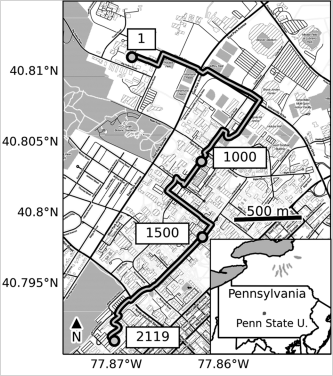
\includegraphics[width=0.5\linewidth]{figures/foresee.png}
    \caption{Map of the FORESEE Array. Photo is taken the PubDAS paper \cite{spica2023pubdas}}
    \label{fig:foresee}
\end{figure}

\begin{table}[!htbp]
    \centering
    \small
    \begin{tabular}{@{}p{0.3\textwidth}p{0.4\textwidth}p{0.2\textwidth}@{}}
        \toprule
        \textbf{Parameter} & \textbf{Value} & \textbf{Unit} \\
        \midrule
        Experiment & Foresee & \\
        Interrogator Unit (IU) & Silixa iDAS-v2 & \\
        Gauge length & 10 & \si{\meter} \\
        Cable length & 23300 & \si{\meter} \\
        Channel spacing & 2 & \si{\meter} \\
        \midrule
        \textbf{Original Data} & & \\
        Format & TDMS & \\
        Samples per second & 500 & \si{\hertz} \\
        File duration & 10 & \si{\minute} \\
        Data shape & 300000 \(\times\) 2137 & \\
        \midrule
        \textbf{After Preprocessing} & & \\
        Format & HDF5 & \\
        Samples per second & 125 & \si{\hertz} \\
        File duration & 5 & \si{\second} \\
        Data shape & 625 \(\times\) 2137 & \\
        \midrule
        \textbf{Dataset Information} & & \\
        Train dataset size & 25690 files & \\
        Train dataset span & 02 Mar 2020 08:10:15 to \newline 03 Mar 2020 20:40:10 & \\
        Labeled dataset size & 600 files & \\
        Labeled dataset span & 15 Apr 2019 03:17:35 to \newline 15 Apr 2019 04:07:30 & \\
        \bottomrule
    \end{tabular}
    \caption{FORESEE Experiment Data Summary}
    \label{tab:foresee_experiment_data}
\end{table}

PubDAS consist of 8 datasets stored in 3 different file formats. These 3 are \texttt{TDMS}, \texttt{HDF5} and \texttt{SEG-Y}. 
The FORESEE

\subsection{Data Preprocessing}

Some preprocessing on the dataset has already been done. This code is highlighted in the appendix \ref{app:pubdas}. To reduce the memory requirements of training such a dataset, we split the files into 5 second intervals compared to the original 10 minutes. Not only does this reduce memory requirements, but anomaly detection may be run every 5 seconds compared to the original 10 minutes. \\

Subsequentially, we chose a test dataset to label anomalies on based on this paper \cite{zhu2023seismic}, that found 18 thunder-induced seismic events in in this timestamp. We manually these data to be able to calculate confusion matrices and other relevant metrics to test the accuracy of our autoencoders. Information about these datasets can be found in table \ref{tab:foresee_experiment_data}. \\

When first downloading these data, they're stored in 10-minute files, resulting in quite large files as shown below:

\begin{align*}
\text{Size} &= 10 \times 60 \times 125 \times 2137 \times 4 \\
&= 600 \times 125 \times 2137 \times 4 \\
&= 641,100,000 \text{ bytes} \\
&\approx 641.1 \text{ MB} \\
&\approx 0.6411 \text{ GB}
\end{align*}

where:
\begin{itemize}
    \item 10 minutes is the duration of each file
    \item 60 seconds per minute
    \item 125\si{\hertz} is the sampling rate
    \item 2137 is the number of channels
    \item 4 bytes per sample (Float32)
\end{itemize}

Most consumer grade \acrshort{gpu}s can only store about 8-16gb of data in VRAM, thus meaning the batches of data we can store is not that big. Additionally, not only does the \acrshort{gpu}s have to store data, but also the weights and biases of the model, as well as losses and more. Motivated by this, we decide to split the files to last 5 seconds compared to 10 minutes. \\ 

We start of by looking at the file names and removing the prefix \textbf{FORESEE\_UTC\_}, since we're only working with one dataset at the time. Furthermore, in parallel fashion, we split each of the files in smaller ones, calculating new filenames based on the beginning timestamp. Now, each \acrshort{hdf5} file store a $625*2137$ matrix of \acrshort{das} data, successfully reducing the memory usage. 
These data are originally stored as \texttt{Float32}, but will be casted as \texttt{Float16} for faster training as we will see later on. In total, more than 25 000 files from the month of april 2020 is gathered to train our model on. 
RESULT: SPEAK ABOUT 5 SECONDS FOR LIVE ENVIRONMENT.
TODO: Inference data from 15042019!


\subsection{Evaluation}

We will be separating the evaluation of \texttt{TinyDAS} into two sections. The first section will focus more on overall model training. Here is a list of points to be evaluated: 

\begin{itemize}
    \item \textbf{Experiment 1}: Median training time and model sizes, and losses
    \item \textbf{Experiment 2}: Reconstruction Capabilities
\end{itemize}

The second section will revolve around anomaly detection based on the different architectures. There are several different methods to evaluate the effectiveness and accuracy of models designed for anomaly detection. A very common pattern is to measure predicted results up against some ground truths, and construct a confusion matrix based on the result. As we saw in listing \ref{code:thresh}. To be able to evaluate the model, we first label ground truths. This is done by iterating over files in a dataset, marking indices of anomalous data to a text file. Furthermore, we will be constructing a confusion 

From this confusion matrix, the following metrics will be used. \\ 


The True Positive Rate (TPR), also known as recall calculated the percentage of truths calculated out of all ground truths. TP is true positives, and FN is false negatives. 

\begin{equation}
    TPR = \frac{TP}{TP + FN} = Recall
\end{equation}
\vspace{0.2cm}

Likewise, the False Positive Rate is the percentage of falsehoolds calculated out of all the ground negatives. FP is false negatives, and TN is true negatives:

\begin{equation}
    FPR = \frac{FP}{FP + TN}
\end{equation}
\vspace{0.2cm}

Precision is the percentage of correct truths out of all predicted truths.

\begin{equation}
    Precision = \frac{TP}{TP + FP}
\end{equation}

\vspace{0.2cm}

The $F1\_{score}$ is used to evaluate the balance between intrusion detection accuracy and recall rate; the higher the score, the better:
\begin{equation}
    F1\_{score} = 2 \times (\frac{Precision \cdot Recall}{Precision + Recall})
\end{equation}

\vspace{0.2cm}

Accuracy measures the proportion of correct predictions:

\begin{equation}
    Accuracy = \frac{TP + TN}{TP + TN + FP + FN}
\end{equation}

\vspace{0.5cm}

For the anomaly detection part of TinyDAS, the following experiments will be conducted

\begin{itemize}
    \item \textbf{Experiment 4}: Anomaly Detection Accuracy
    \item \textbf{Experiment 5}: Confusion Matrix and Metrics
\end{itemize}


\subsection{Experiment Setup}

All the models were trained and tested on \gls{idun} computers made for \acrshort{hpc}. Configuration parameter for the different models can be found in the appendix \ref{app:judasnethyperparams}, and details of the machines used can be found in the table below. \\


\begin{table}[!htbp]
\centering
\caption{Specifications for Model Training and Testing Environment}
\label{tab:system-specs}
\begin{tabular}{@{}llr@{}}
\toprule
\textbf{Component} & \textbf{Description} & \textbf{Quantity} \\
\midrule
Operating System & Ubuntu Linux 22.04 LTS & 1 machine \\
GPU Model & NVIDIA H100 PCIe & 4 units \\
GPU Memory & HBM3 & 80 GB per GPU \\
CUDA Cores & & 14,592 per GPU \\
Tensor Cores & & 576 per GPU \\
GPU Clock Speed & Boost Clock & 1.67 GHz \\
GPU TDP & & 350 W \\
FP16 & & 204.9 TFLOPS \\
FP32 & & 51.22 TFLOPS \\
\midrule
\multicolumn{3}{@{}l@{}}{\textit{Note:} 1 \acrshort{gpu} dedicated for testing, 4 for training.} \\
\bottomrule
\end{tabular}
\end{table}



\chapter{Experimental Results}
\label{chap:results}

This fourth chapter presents the results from the experiments introduced in chapter \ref{chap:exp}. 


\section{BANENOR}
\label{res:Judas}


\subsection{Experiment \rnum{1}: HDF5 file processing and resampling}

In this experiment, we will be processing $n$ amount of \acrshort{hdf5} files with $p$ processes, from the point of reading raw data gathered by \acrshort{cgf} from the OptoDAS, through pre-processing, resampling the signals and denoising the result. This will give an accurate view of what needs to happen from rawdata until they are ready to be trained on different \acrshort{ml} or \acrshort{dl} models. Full code example can be found in appendix \ref{app:judas}. \\

We will be resampling the signals to $100Hz$ from $500Hz$, and the Channel ROI will be 250m. We will be utilizing 1, 2, 4 and 8 processes, and use of a different amount of \acrshort{das} data ranging from 10 seconds until 1 hour of \acrshort{das} data.

\begin{figure}[!h]
    \centering
    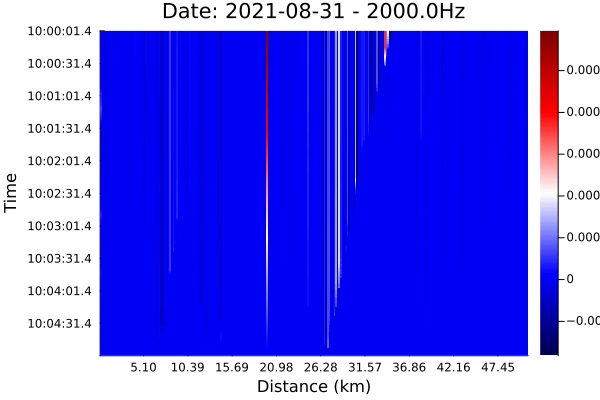
\includegraphics[width=0.8\linewidth]{figures/heatmap_das_test.png}
    \caption{Heatmap of the processed data before resampling and denoising}
    \label{fig:dasoutput}
\end{figure}



\begin{figure}[!htbp]
\centering
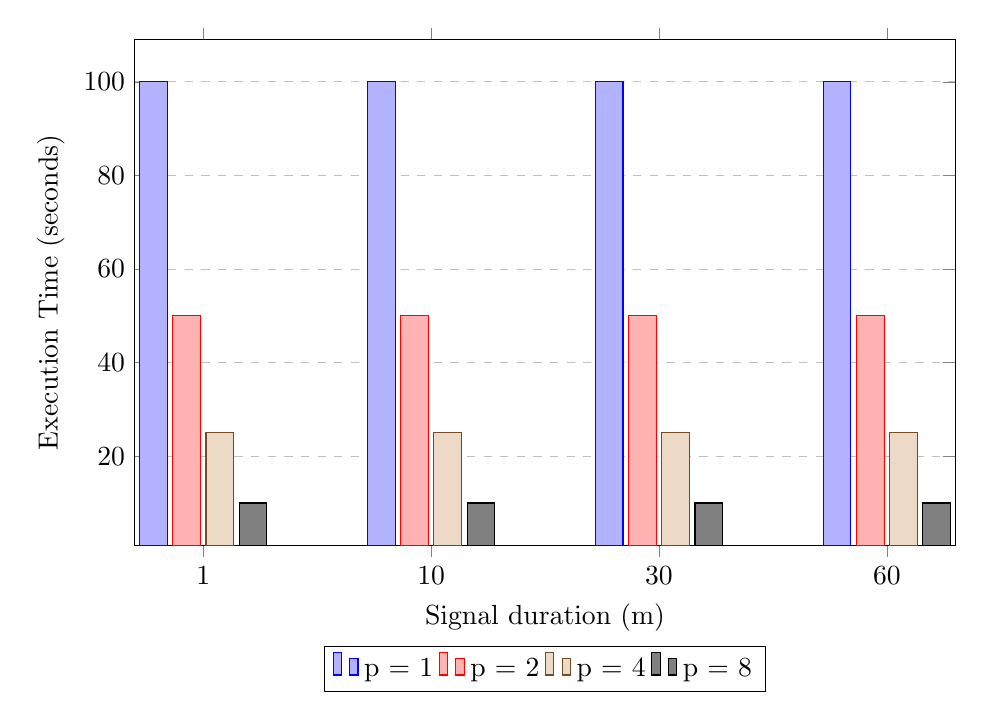
\begin{tikzpicture}
\begin{axis}[
    ylabel={Execution Time (seconds)},
    xlabel={Signal duration (m)},
    xticklabels={1,10, 30, 60},
    xtick={1,10,30,60},
    legend pos=north west,
    ymajorgrids=true,
    grid style=dashed,
    width=12cm,
    height=8cm,
    bar width=10pt,
    ybar,
    legend style={at={(0.5,-0.20)},
    anchor=north,legend columns=-1},
    symbolic x coords={1, 10, 30, 60},
]
\addplot coordinates {(1,100)(10,100)(30,100)(60,100) };
\addplot coordinates {(1,50) (10,50) (30,50) (60,50) };
\addplot coordinates {(1,25) (10,25) (30,25) (60,25) };
\addplot coordinates {(1,10) (10,10) (30,10) (60,10) };
\legend{p = 1, p = 2, p = 4, p = 8}
\end{axis}
\end{tikzpicture}
\caption{Execution times for different problem sizes and process counts}
\label{fig:judas-benchmark}
\end{figure}

As we can see.

\begin{figure}[!htbp]
\centering
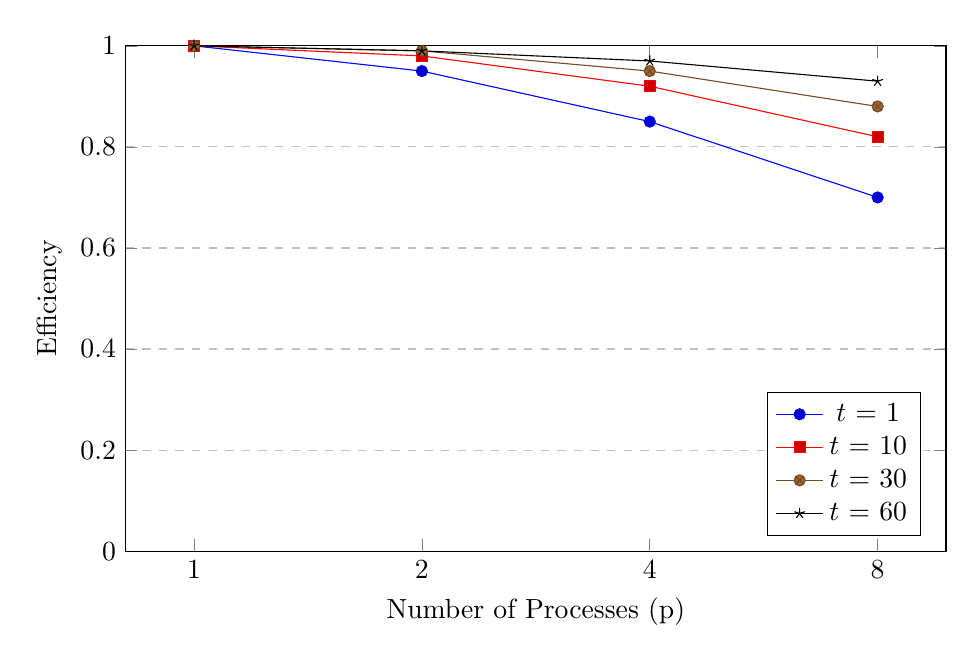
\begin{tikzpicture}
\begin{axis}[
    ylabel={Efficiency},
    xlabel={Number of Processes (p)},
    xticklabels={1,2,4,8},
    xtick={1,2,3,4},
    legend pos=south east,
    ymajorgrids=true,
    grid style=dashed,
    width=12cm,
    height=8cm,
    ymax=1,
    ymin=0,
]
\addplot coordinates {(1,1) (2,0.95) (3,0.85) (4,0.70)};
\addplot coordinates {(1,1) (2,0.98) (3,0.92) (4,0.82)};
\addplot coordinates {(1,1) (2,0.99) (3,0.95) (4,0.88)};
\addplot coordinates {(1,1) (2,0.99) (3,0.97) (4,0.93)};
\legend{$t$ = 1, $t$ = 10, $t$ = 30, $t$ = 60}
\end{axis}
\end{tikzpicture}
\caption{Efficiency for different problem sizes and process counts. $m$ is the amount of minutes of data we want to process.}
\label{fig:efficiency}
\end{figure}

\subsection{Experiment \rnum{2}: Parallel Resampling}

For this experiment, we will be using the same signals as we did in our last experiment. The duration of the \acrshort{das} signal will be 5 minutes, meaning the input matrix will be of size $600000
\times 261$ We will be resampling to $1000Hz, 500Hz, 250Hz, 100Hz$, utilizing 1, 2, 4 and 8 processes. For this operation \\



\begin{figure}[!htbp]
\centering
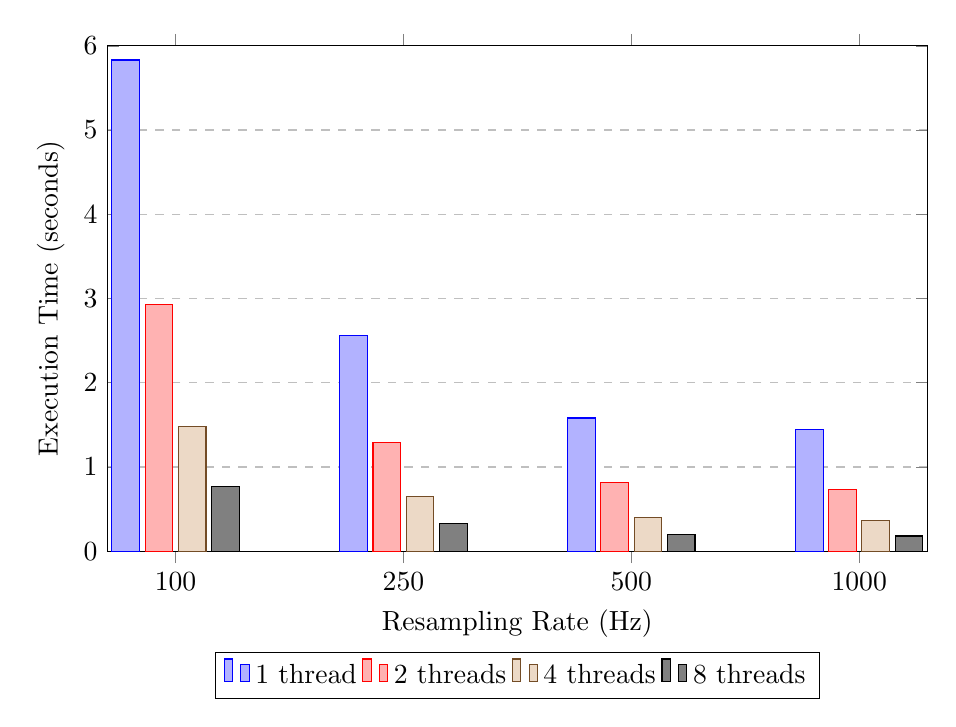
\begin{tikzpicture}
\begin{axis}[
    ylabel={Execution Time (seconds)},
    xlabel={Resampling Rate (Hz)},
    xticklabels={1000, 500, 250, 100},
    xtick={1000,500,250,100},
    legend pos=north west,
    ymajorgrids=true,
    grid style=dashed,
    width=12cm,
    height=8cm,
    bar width=10pt,
    ybar,
    legend style={at={(0.5,-0.20)},
    anchor=north,legend columns=-1},
    symbolic x coords={1000, 500, 250, 100},
    x dir=reverse,
    ymin=0, ymax=6,
]
\addplot coordinates {(1000,1.448) (500,1.581) (250,2.563) (100,5.832)};
\addplot coordinates {(1000,0.732) (500,0.817) (250,1.286) (100,2.928)};
\addplot coordinates {(1000,0.363) (500,0.400) (250,0.650) (100,1.478)};
\addplot coordinates {(1000,0.181) (500,0.200) (250,0.325) (100,0.772)};
\legend{1 thread, 2 threads, 4 threads, 8 threads}
\end{axis}
\end{tikzpicture}
\caption{Execution times for different resampling rates and thread counts}
\label{fig:resampling-benchmark}
\end{figure}


\begin{figure}[!htbp]
\centering
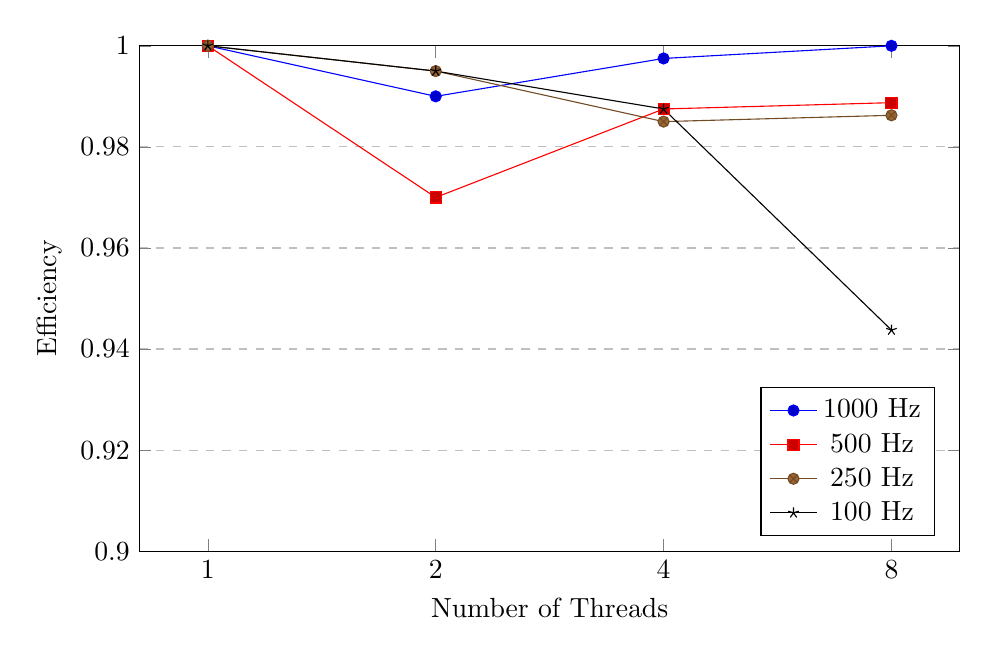
\begin{tikzpicture}
\begin{axis}[
    ylabel={Efficiency},
    xlabel={Number of Threads},
    xticklabels={1,2,4,8},
    xtick={1,2,3,4},
    legend pos=south east,
    ymajorgrids=true,
    grid style=dashed,
    width=12cm,
    height=8cm,
    ymax=1,
    ymin=0.90,
]
\addplot coordinates {(1,1) (2,0.99) (3,0.9975) (4,1.00)};
\addplot coordinates {(1,1) (2,0.97) (3,0.9875) (4,0.98875)};
\addplot coordinates {(1,1) (2,0.995) (3,0.985) (4,0.98625)};
\addplot coordinates {(1,1) (2,0.995) (3,0.9875) (4,0.94375)};
\legend{1000 Hz, 500 Hz, 250 Hz, 100 Hz}
\end{axis}
\end{tikzpicture}
\caption{Efficiency for different resampling rates and thread counts}
\label{fig:resampling_efficiency}
\end{figure}

Figure \ref{fig:resampling-benchmark} clearly indicates how the addition of more processes decreases the overall runtime of the function. Lower resampling, and overall smaller resampling rate, obviously increase the overall time, yet even here, the average wall time for resampling to $100Hz$ using 8 threads only use about 0.8 seconds. \\


As we can see from figure \ref{fig:resampling_efficiency}, we achieve high efficiency, and near-linear scaling for all rates and frequencies. The only notable drop happens at $100Hz$ using 8 threads, but we still achieve an efficiency of around 0.94. 
\section{FORESEE}
\label{res:tinydas}


\subsection{Experiment \rnum{1}: Model training and Reconstruction}

As we can see in the table ...




\begin{table}[!htbp]
    \centering
    \begin{tabular}{lcccc}
        \hline
        \textbf{Metric} & \textbf{AE} & \textbf{CAE} & \textbf{VAE} & \textbf{CVAE} \\
        \hline
        Best loss & 1.3e-6 & 0.032 & 0.038 & 0.029 \\
        Epochs before stop & 6 & 20 & 15 & 15 \\
        \hline
    \end{tabular}
    \caption{Comparison of Autoencoder Performance\\ *The Reconstruciton error is the sum of all reconstruction errors across all batches.}
    \label{tab:autoencoder_comparison}
\end{table}

\begin{figure}[!h]
    \centering
    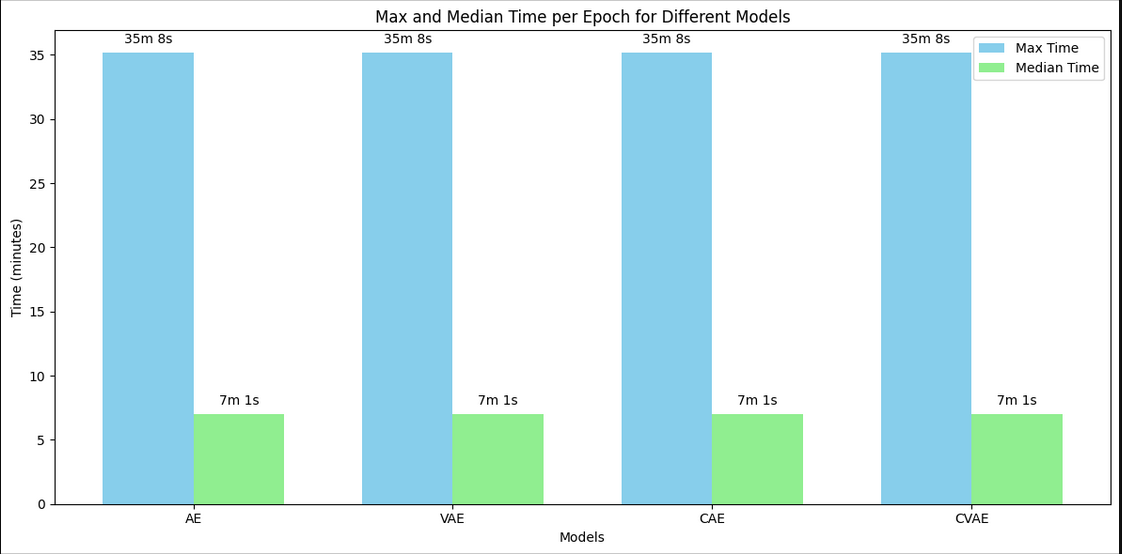
\includegraphics[scale=0.4]{figures/time.png}
    \caption{Training times}
    \label{fig:traintimes}
\end{figure}

As we can see in figure \ref{fig:traintimes}, there is a huge difference between the max training time and the median training time. The max training time always happens during the first epoch, when the \texttt{train\_step} and \texttt{val\_step} kernels are being compiled. Total training times per model are all under \qty{6}{\si{\hour}} before the training is stopped early due to the \textit{early stopping} mechanism.

\subsubsection{Loss Values}

The following is a list of how the losses changed over time...


\begin{figure}[!htbp]
  \centering
  \begin{subfigure}[t]{.6\textwidth}
    \centering
    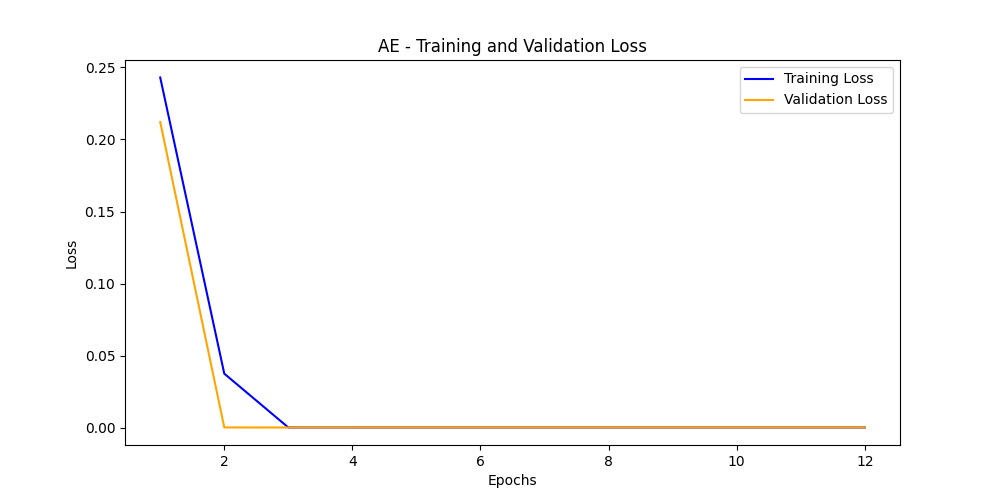
\includegraphics[width=\linewidth]{figures/losses/ae.png}
    \caption{AE}
  \end{subfigure}
  \hfill
  \begin{subfigure}[t]{.6\textwidth}
    \centering
    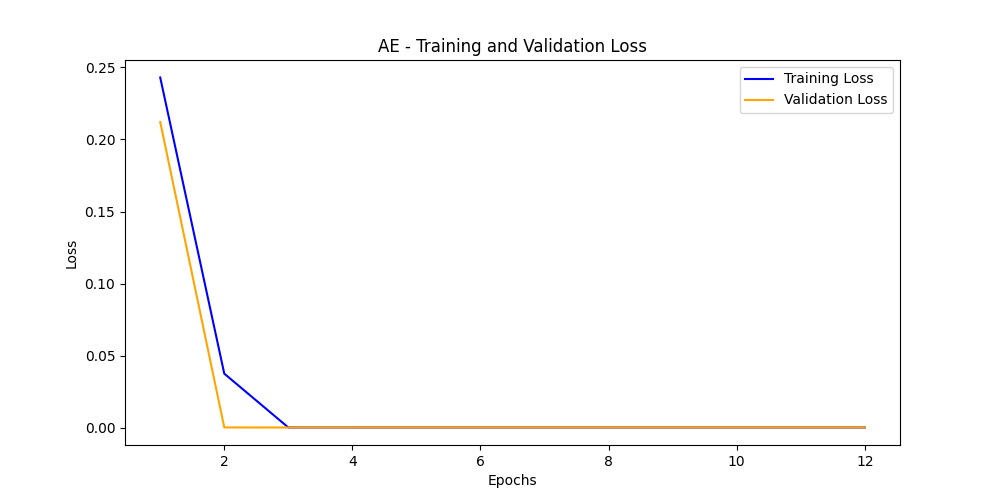
\includegraphics[width=\linewidth]{figures/losses/ae.png}
    \caption{CAE}
  \end{subfigure}
  
  \vspace{1cm}
  
  \begin{subfigure}[t]{.6\textwidth}
    \centering
    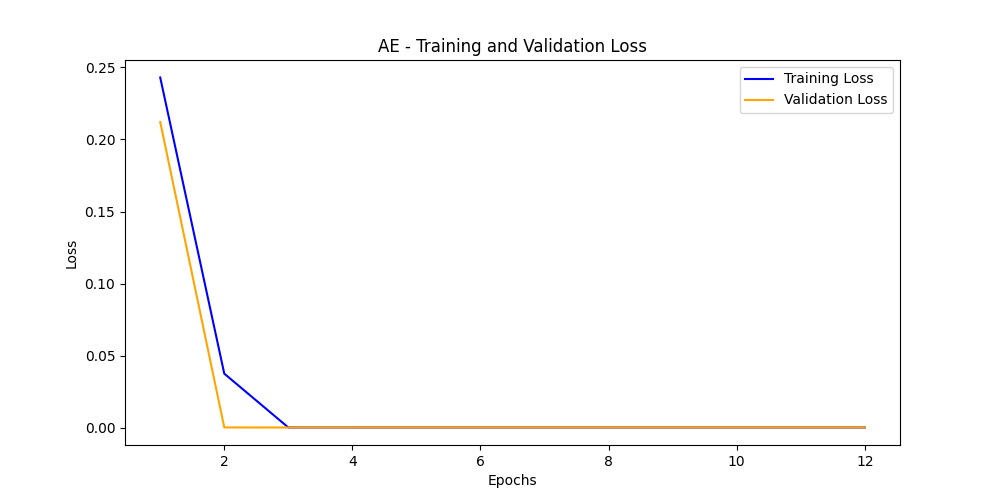
\includegraphics[width=\linewidth]{figures/losses/ae.png}
    \caption{VAE}
  \end{subfigure}
  \hfill
  \begin{subfigure}[t]{.6\textwidth}
    \centering
    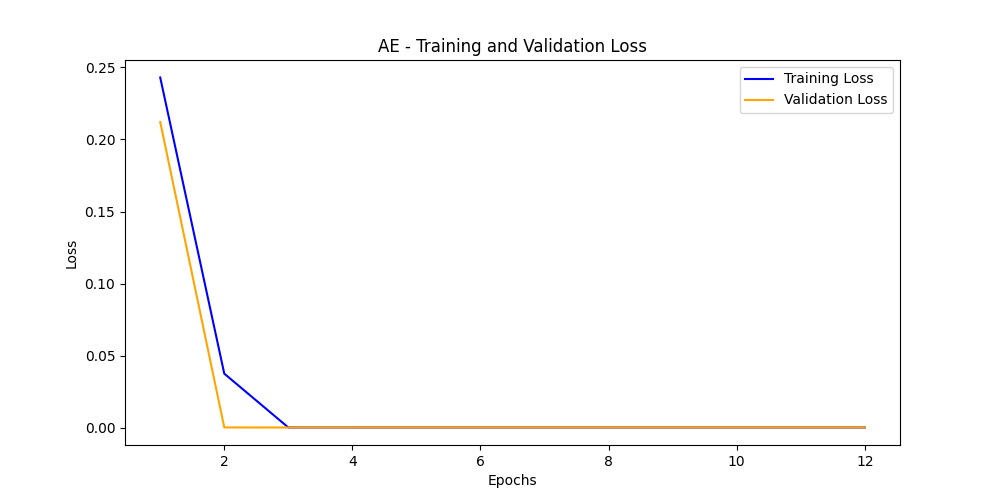
\includegraphics[width=\linewidth]{figures/losses/ae.png}
    \caption{CVAE}
  \end{subfigure}
  \caption{Train and Validation Loss per epoch}
\end{figure}

\subsubsection{Reconstruction Capabiltites}

\begin{figure}[!h]
    \centering    
    % Row 0 (Image Names)
    \begin{subfigure}{0.33\textwidth}
        \centering
        \textbf{Image 1}
    \end{subfigure}%
    \hfill
    \begin{subfigure}{0.33\textwidth}
        \centering
        \textbf{Image 2}
    \end{subfigure}%
    \hfill
    \begin{subfigure}{0.33\textwidth}
        \centering
        \textbf{Image 3}
    \end{subfigure}
    
    \vspace{1em}
    
    % Row 1 (Original)
    \begin{subfigure}{0.33\textwidth}
        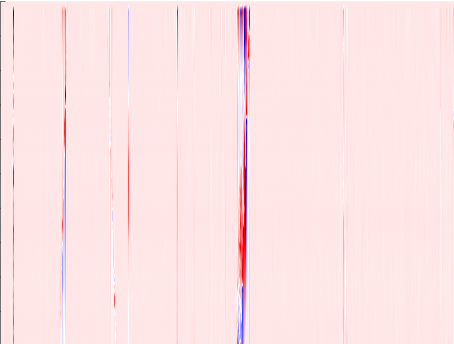
\includegraphics[width=\textwidth]{figures/test.png}
        \caption{Original}
    \end{subfigure}%
    \hfill
    \begin{subfigure}{0.33\textwidth}
        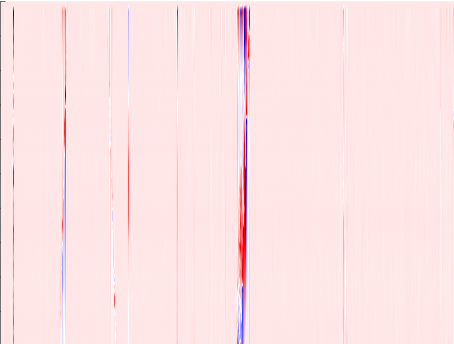
\includegraphics[width=\textwidth]{figures/test.png}
        \caption{Original}
    \end{subfigure}%
    \hfill
    \begin{subfigure}{0.33\textwidth}
        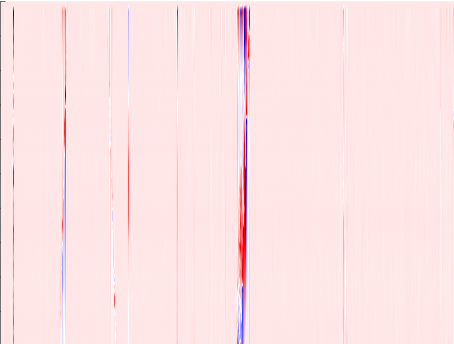
\includegraphics[width=\textwidth]{figures/test.png}
        \caption{Original}
    \end{subfigure}
    
    \vspace{1em}
    
    % Row 2 (Model 1)
    \begin{subfigure}{0.33\textwidth}
        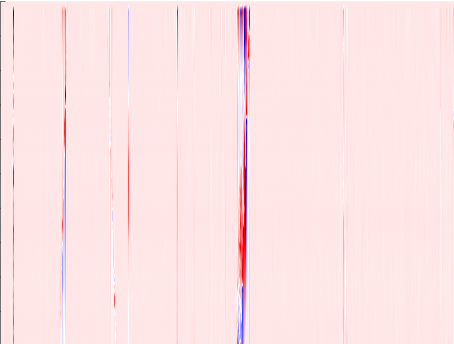
\includegraphics[width=\textwidth]{figures/test.png}
        \caption{AE}
    \end{subfigure}%
    \hfill
    \begin{subfigure}{0.33\textwidth}
        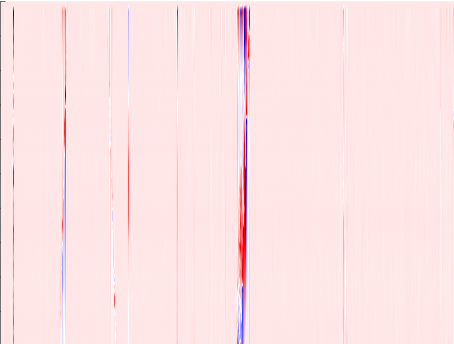
\includegraphics[width=\textwidth]{figures/test.png}
        \caption{AE}
    \end{subfigure}%
    \hfill
    \begin{subfigure}{0.33\textwidth}
        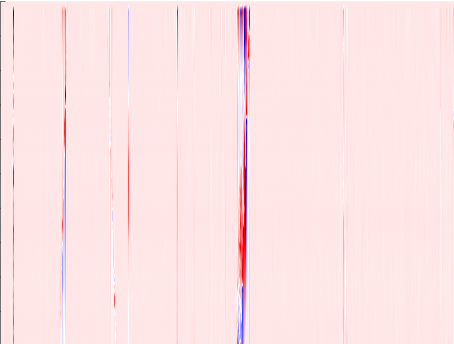
\includegraphics[width=\textwidth]{figures/test.png}
        \caption{AE}
    \end{subfigure}
    
    \vspace{1em}
    
    % Row 3 (Model 2)
    \begin{subfigure}{0.33\textwidth}
        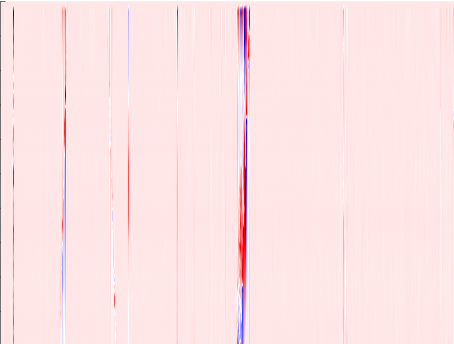
\includegraphics[width=\textwidth]{figures/test.png}
        \caption{CAE}
    \end{subfigure}%
    \hfill
    \begin{subfigure}{0.33\textwidth}
        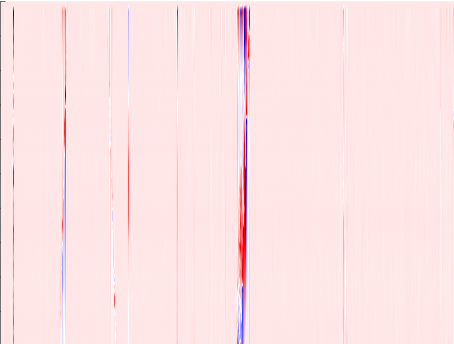
\includegraphics[width=\textwidth]{figures/test.png}
        \caption{CAE}
    \end{subfigure}%
    \hfill
    \begin{subfigure}{0.33\textwidth}
        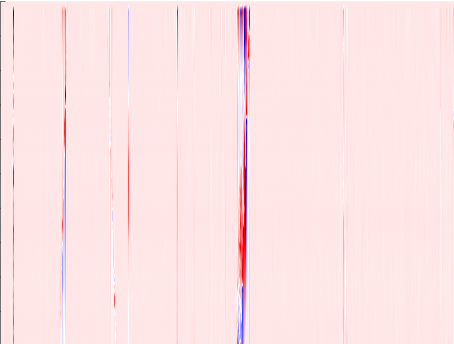
\includegraphics[width=\textwidth]{figures/test.png}
        \caption{CAE}
    \end{subfigure}
    
    \vspace{1em}
    
    % Row 4 (Model 3)
    \begin{subfigure}{0.33\textwidth}
        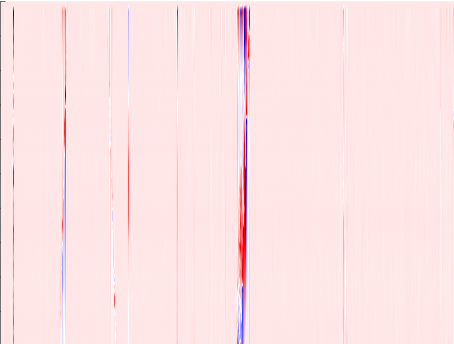
\includegraphics[width=\textwidth]{figures/test.png}
        \caption{VAE}
    \end{subfigure}%
    \hfill
    \begin{subfigure}{0.33\textwidth}
        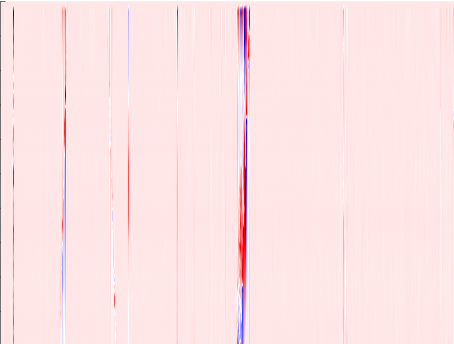
\includegraphics[width=\textwidth]{figures/test.png}
        \caption{VAE}
    \end{subfigure}%
    \hfill
    \begin{subfigure}{0.33\textwidth}
        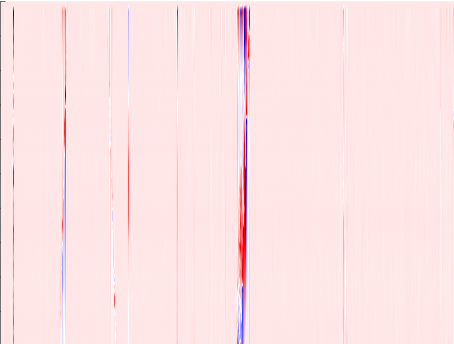
\includegraphics[width=\textwidth]{figures/test.png}
        \caption{VAE}
    \end{subfigure}
    
    \vspace{1em}
    
    % Row 5 (Model 4)
    \begin{subfigure}{0.33\textwidth}
        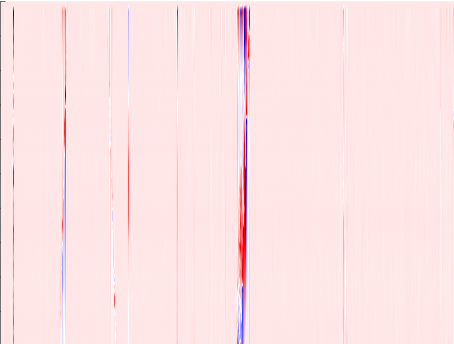
\includegraphics[width=\textwidth]{figures/test.png}
        \caption{CVAE}
    \end{subfigure}%
    \hfill
    \begin{subfigure}{0.33\textwidth}
        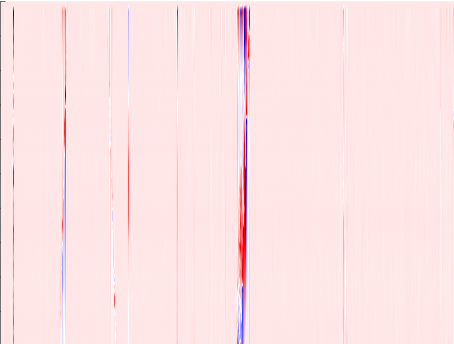
\includegraphics[width=\textwidth]{figures/test.png}
        \caption{CVAE}
    \end{subfigure}%
    \hfill
    \begin{subfigure}{0.33\textwidth}
        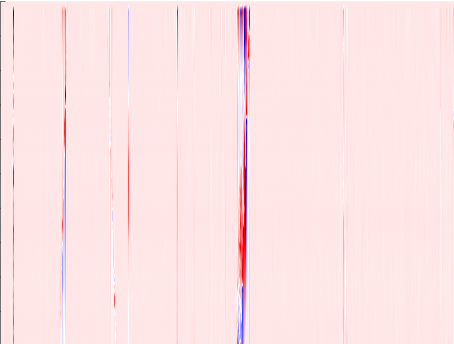
\includegraphics[width=\textwidth]{figures/test.png}
        \caption{CVAE}
    \end{subfigure}
    
    \caption{Comparison of original images and their reconstructions by different autoencoders}
    \label{fig:aereconstruct}
\end{figure}

\subsection{Experiment \rnum{2}: Anomaly Detection}

An important part of analysing our autoencoders is the choice of metrics. Whereas loss and accuracy can provide proficient details about the model training itself, other metrics are better suited for analysing the 

Table \ref{tab:autoencoder_comparison} presents a comparative analysis of the four autoencoder types: dense, convolutional, variational dense, and variational convolutional.





% Confusion Matrix Components Table
\begin{table}[!htbp]
\centering
\label{tab:confusion-matrix-results}
\begin{tabular}{l
    S[table-format=3.0]
    S[table-format=3.0]
    S[table-format=3.0]
    S[table-format=3.0]
    S[table-format=3.2]
    S[table-format=3.2]
}
\toprule
\textbf{Model} & {\textbf{TP}} & {\textbf{FP}} & {\textbf{TN}} & {\textbf{FN}} & {\textbf{Precision (\%)}} & {\textbf{Recall (\%)}} \\
\midrule
\rowcolor{gray!10} AE   & 100 & 10 & 80 & 10 & 90.91 & 90.91 \\
CAE  & 95 & 15 & 75 & 15 & 86.36 & 86.36 \\
\rowcolor{gray!10} VAE  & 105 & 8 & 85 & 5 & 92.92 & 95.45 \\
CVAE & 30 & 110 & 460 & 0 & 21.43 & 100.00 \\
\bottomrule
\end{tabular}
\caption{Confusion Matrix Components and Derived Metrics}
\end{table}


% Performance Metrics Table

\begin{table}[!htbp]
\centering
\label{tab:performance-metrics}
\begin{tabular}{l
    S[table-format=1.3]
    S[table-format=1.3]
    S[table-format=1.3]
    S[table-format=1.3]
    S[table-format=1.3]
}
\toprule
\textbf{Model} & {\textbf{TPR}} & {\textbf{FPR}} & {\textbf{Precision}} & {\textbf{F1-Score}} & {\textbf{Accuracy}} \\
\midrule
\rowcolor{gray!10} AE   & 0.909 & 0.111 & 0.909 & 0.909 & 0.900 \\
CAE  & 0.864 & 0.167 & 0.864 & 0.864 & 0.850 \\
\rowcolor{gray!10} VAE  & 0.955 & 0.086 & 0.929 & 0.942 & 0.941 \\
CVAE & 0.910 & 0.128 & 0.910 & 0.900 & 0.817 \\
\bottomrule
\end{tabular}
\caption{Model Performance Metrics Comparison}
\end{table}

\begin{figure}[!h]
\centering
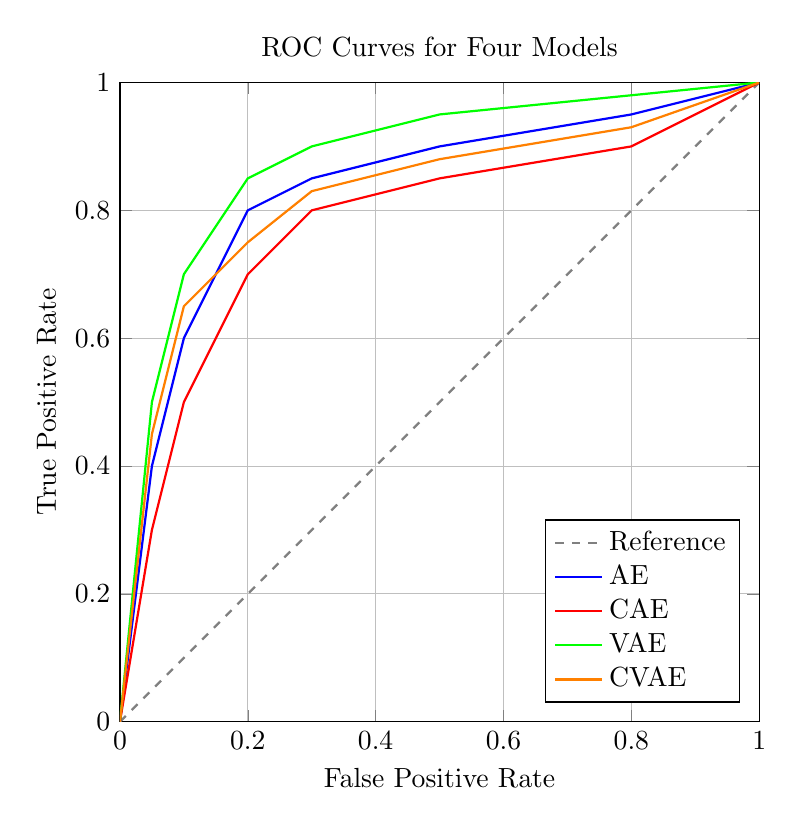
\begin{tikzpicture}
\begin{axis}[
    width=0.8\textwidth,
    height=0.8\textwidth,
    xlabel={False Positive Rate},
    ylabel={True Positive Rate},
    xmin=0, xmax=1,
    ymin=0, ymax=1,
    xtick={0,0.2,0.4,0.6,0.8,1},
    ytick={0,0.2,0.4,0.6,0.8,1},
    legend pos=south east,
    legend cell align={left},
    grid=major,
    title={ROC Curves for Four Models}
]

% Diagonal reference line
\addplot[thick,dashed,gray] coordinates {(0,0) (1,1)};

% ROC curve for Model A
\addplot[thick,blue] coordinates {
    (0,0) (0.05,0.4) (0.1,0.6) (0.2,0.8) (0.3,0.85) (0.5,0.9) (0.8,0.95) (1,1)
};

% ROC curve for Model B
\addplot[thick,red] coordinates {
    (0,0) (0.05,0.3) (0.1,0.5) (0.2,0.7) (0.3,0.8) (0.5,0.85) (0.8,0.9) (1,1)
};

% ROC curve for Model C
\addplot[thick,green] coordinates {
    (0,0) (0.05,0.5) (0.1,0.7) (0.2,0.85) (0.3,0.9) (0.5,0.95) (0.8,0.98) (1,1)
};

% ROC curve for Model D
\addplot[thick,orange] coordinates {
    (0,0) (0.05,0.45) (0.1,0.65) (0.2,0.75) (0.3,0.83) (0.5,0.88) (0.8,0.93) (1,1)
};

\legend{Reference, AE, CAE, VAE, CVAE}

\end{axis}
\end{tikzpicture}
\caption{ROC Curves Comparison for our Autoencoders }
\end{figure}

\begin{figure}[!h]
\centering
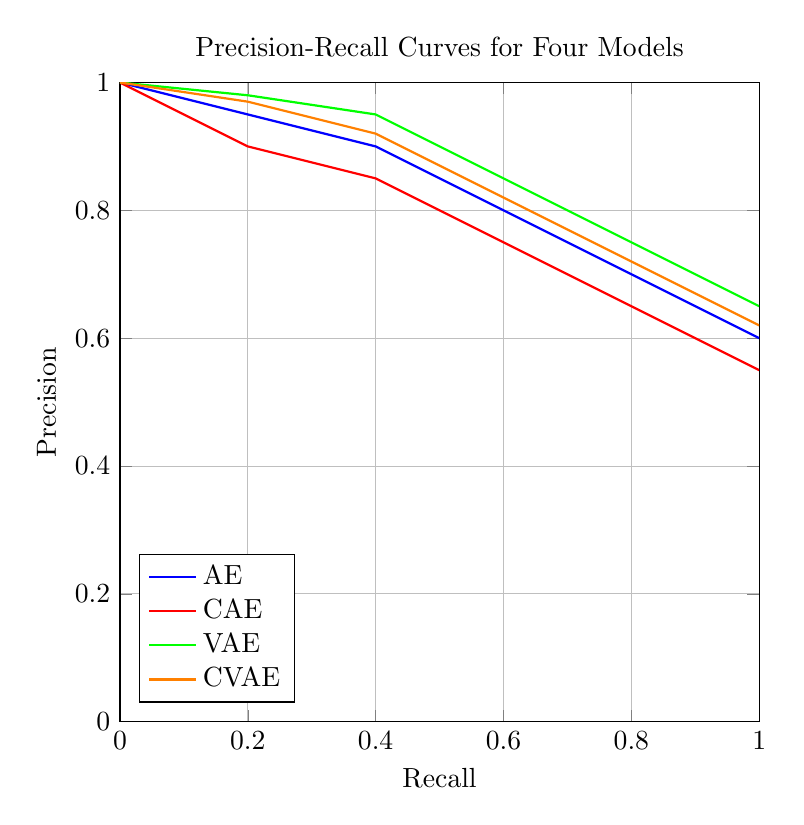
\begin{tikzpicture}
\begin{axis}[
    width=0.8\textwidth,
    height=0.8\textwidth,
    xlabel={Recall},
    ylabel={Precision},
    xmin=0, xmax=1,
    ymin=0, ymax=1,
    xtick={0,0.2,0.4,0.6,0.8,1},
    ytick={0,0.2,0.4,0.6,0.8,1},
    legend pos=south west,
    legend cell align={left},
    grid=major,
    title={Precision-Recall Curves for Four Models}
]
% PR curve for Model AE
\addplot[thick,blue] coordinates {
    (0,1) (0.2,0.95) (0.4,0.9) (0.6,0.8) (0.8,0.7) (1,0.6)
};
% PR curve for Model CAE
\addplot[thick,red] coordinates {
    (0,1) (0.2,0.9) (0.4,0.85) (0.6,0.75) (0.8,0.65) (1,0.55)
};
% PR curve for Model VAE
\addplot[thick,green] coordinates {
    (0,1) (0.2,0.98) (0.4,0.95) (0.6,0.85) (0.8,0.75) (1,0.65)
};
% PR curve for Model CVAE
\addplot[thick,orange] coordinates {
    (0,1) (0.2,0.97) (0.4,0.92) (0.6,0.82) (0.8,0.72) (1,0.62)
};
\legend{AE, CAE, VAE, CVAE}
\end{axis}
\end{tikzpicture}
\caption{Precision-Recall Curves Comparison for our Autoencoders}
\end{figure}




Clearbout \cite{claerbout1991scrutiny}
Landes scrutiny \cite{landes1951scrutiny}
omar2013 machine \cite{omar2013machine}
wei lstm autoenc \cite{wei2022lstmautoencoder}
apsensing railways \cite{apSensing2019railwaydas}
srivatavams15 \cite{DBLP:journals/corr/SrivastavaMS15}
2011 ndonssigprocandet \cite{2011ndongsigprocandet}
doi101136141000671 \cite{doi:10.1137/141000671}
bioeng \cite{bioengineering10040405}
maulik2020recurr \cite{maulik2020recurrent}





\chapter{Discussion}
\label{chap:disc}

This sixth chapter analyzes the results presented in Chapter \ref{chap:results} and further examines the programs detailed in Chapter \ref{chap:exp}. We explore the overall design, strengths, and current limitations of both \texttt{Judas} and \texttt{TinyDAS}. The chapter concludes with an evaluation of Julia as a programming language for data science and \acrshort{ai} applications.


%%\subsection{Did we reach our goals?}


\textbf{G1: Evaluate the effectiveness in detecting anomalies within \acrshort{das} data}. With our autoencoder based approach, we're able to effectively detecting anomalies within \acrshort{das} data. With even bigger datasets, and more image labeling of \acrshort{das} data, we believe one can achieve even greater results. \\

\textbf{G2: Contribute to the open source community, particularly with tools and resources that are beneficial to members of \acrshort{cgf}.} Throughout our work, we've always maintained a strong stance on developing tools that are both beneficial and easy to use. We firmly believe that both of our tools can be of use, specifically for members at \acrshort{cgf}.  \\ 

\textbf{G3: Determine whether Julia is a suitable programming language for 
 high performance data processing, analysis and \acrshort{ai}, specifically aimed at \acrshort{das} data}. Overall, we find Julia satisfactory in developing novel, high performance algorithms, as well as working with data science in general, yet lacking when it comes to training \acrshort{ai} models across multiple \acrshort{gpu}s. We believe it to be an effective language of choice for members at \acrshort{cgf}.\\



\section{BANENOR}
\label{disc:banenor}

\subsection{Experiment \rnum{1}: Data processing and resampling}

Analysis of the current processing pipeline reveals significant bottlenecks in the \texttt{load\_DAS\_files} function. Figure \ref{fig:judasextime} clearly demonstrates that loading the \acrshort{hdf5} files represents the bottleneck of of our approach. This largely stems from our fine-grained approach to parallelization within the \texttt{load\_DAS\_files} function. While we have implemented parallel processing techniques in specific parts of this function, the overwhelming majority of this function is strictly serial. The efficiency issues are further illustrated by Figure \ref{fig:judasefficiency}, showcasing a marked decline in processing efficiency across all time windows and durations.
Following the parallel loading phase, the function encounters another slowdown as it waits for the \texttt{ccds!} function to finish. This sequential processing step further hinders the overall performance limitations of our current implementation.
Despite these challenges, our approach of fine-grained parallelization within \texttt{load\_DAS\_files} and using memory mapping for signal data to binary files has provided valuable insights. These findings strongly indicate the necessity for a comprehensive overhaul of the current IO operations to fully leverage parallel techniques and reduce overall runtime.

Even if our approach to file loading proves ineffective, our method offers several advantages. Notably, it eliminates the need for repeated file loading, allowing users to load the required files for initial \acrshort{das} processing and then combine submatrices temporarily stored in binary files for further analyses. This approach reduces redundant data operations and increases overall flexibility. Furthermore, compared to similar programs at \acrshort{cgf}, our implementation substantially reduces overall RAM usage.

While our current implementation faces performance challenges, particularly in file loading and parallel efficiency, it has laid the groundwork for future optimizations. One potential improvement is to parallelize the entire \texttt{load\_DAS\_files} function, where each process $p$ only processes a subset of the filenames returned by the \texttt{find\_DAS\_file} function. This requires a parallel approach to the cumulative summation of submatrices, which the \texttt{ccds!} function currently does not support.


\subsection{Experiment \rnum{2}: Parallel Resampling}

\label{fig:resampling-benchmark}
The overall runtimes displayed in Figure \ref{fig:resampling-benchmark} show a significant improvement for all resampling rates and process counts compared to the serial execution. The runtime decreases by approximately a factor of 2 when moving from serial execution to our parallel version using 2 processes.

Figure \ref{fig:ex2heat} indicates that higher resampling rates benefit more from parallelization compared to lower ones. As expected, using only a single process with our parallel solution introduces minimal overhead, primarily from allocating the shared matrix to the parent process.

The sharp decline in efficiencies, shown in Figure \ref{fig:resampling_efficiency}, indicates strong diminishing returns as the number of processes increases. The most significant decline occurs between 4 and 8 processes, suggesting a potential bottleneck. Compared to the original \acrshort{das} signal matrix with 12500 channels, the overhead of spawning many processes for only 261 channels proves inefficient, particularly for lower resampling rates. This highlights that each process benefits from having a substantial workload, possibly due to Julia's function precompilation, as explained in Section \ref{meth:julia}. 

Our current implementation of parallel resampling does not utilize \acrshort{gpu}s. A potential improvement could be achieved by leveraging \texttt{CUDA.jl} to develop a GPU-accelerated resampling method that takes advantage of existent processing capabilities at \acrshort{cgf}, as shown in table \ref{tab:cgfsetup}. Efficient resampling algorithms for \acrshort{gpu}s have already been demonstrated, for instance, the work by Kim et al. (2013) \cite{kim2013efficient}.

Overall, this experiment demonstrates that our implementation of parallel channel decimation is best suited for more compute-intensive tasks, such as higher resampling rates. For this particular example, the optimal process count appears to be 4 processes, balancing improved performance with efficient resource utilization. Tests across multiple matrix sizes are needed to evaluate the amount of processes necessary further.
\section{FORESEE}
\label{disc:foresee}

\subsection{Experiment \rnum{1}: }
\subsection{Experiment \rnum{2}: }
\section{Judas}
\label{disc:judas}

The improvements to Judas have proved meaningful. The added channel selection lets the user choose which channels to analyze, while the \texttt{load\_DAS\_files} function now utilizes memory mapping, and the processing is done in parallel. The added functionalities of parallel channel decimation, denoising, and other utilities let users further process and analyze \acrshort{das} data. Judas can thus be incorporated into other Julia programs to allow for further analysis. \\

From experiment \rnum{2}, we can clearly see that the current bottleneck of \texttt{Judas} is the first part of the program, more specifically, the \texttt{load\_DAS\_files} function. Even though we successfully avoid loading large arrays into memory by utilizing memory mapping and temporary file storage, only a small part of the function is parallelizable. Nor does it take advantage of Julia's \textit{just-ahead-of-time} compilations, besides the cumulative sum calculation and the parallelized section, which are being called multiple times. A further improved version of loading the files may be needed. This program is also limited to \acrshort{hdf5} files as of now, and metadata for BANENOR datasets. Certain hardcoded values may need modification to make Judas usable for other experiments, but users can make changes themselves wherever necessary. \\

This, of course, limits the effectiveness and scalability of the program. Still, compared to similar programs at \acrshort{cgf}, users can now find and load several \acrshort{das} files over larger durations and utilize multiple processes to speed up the loading of larger matrices. For shorter windows, existing programs prove more effective. \\

Additionally, this first part of the program could be run before resampling and denoising, thus circumventing the need to wait for pre-processing data. An alternative to our fine-grained approach at parallelization would be to parallelize both the \texttt{find\_DAS\_files} and the \texttt{load\_DAS\_files} function. This more coarse-grained approach distributes the files found by \texttt{find\_DAS\_files} across several processes and decreases the overall run time of \texttt{load\_DAS\_files}.\\

Not much effort is necessary to load and analyze \acrshort{das} data. In approximately 30 lines, users can find, load, and process their data and visualize the results. This simplicity and efficiency make Judas a powerful tool for members at \acrshort{cgf} working with \acrshort{das} data.


%There are still plenty of undiscovered methods on this kind of data. As mentioned in \cite{MALEKI2021107443}, "Anomaly detection in unlabelled Big Data is difficult and costly". We've seen this occur even after multiple different rounds of resampling, channel decimation, and so on. 
\section{JudasNET}
\label{disc:judasnet}

After the creation of Judas, we were determined to continue the implementation of \acrshort{ai} models and anomaly detection in Julia. We wanted to train our models on the same dataset as described earlier \ref{met:judas}. Ultimately, there were two reasons for us turning away from Julia and opting for Python instead. \\

The first reason is the limited amount of \acrshort{gpu}s available at \acrshort{cgf}. With only a single consumer grade level \acrshort{gpu} with 11Gb VRAM available, we would have to use smaller batches of data, and maybe decrease window duration. This constraint led us to switch to the \gls{idun} cluster for computation, but we were now not allowed to continue our work on the BANENOR dataset due to it being proprietary and classified data. IDUN is a public server, and most of the data at \acrshort{cgf} is not allowed on public servers. This led us to work with the PubDAS dataset. \\

Even after switching servers and datasets, we could still use Julia and \texttt{Flux.jl} to train our models. The issue here was the core support for multiple training provided by \texttt{Flux.jl}. This issue is being discussed by the maintainers \href{https://github.com/FluxML/Flux.jl/issues/1829}{in a forum}, but ultimately, only third-party solutions exist as of now. Several of these packages are old and are not compatible with current versions of Julia, Flux, or other packages. Instead of implementing this feature ourselves, we want to highlight how autoencoders can be used for anomaly detection on \acrshort{das} data, and thus, we ended up going with Python in the end. 

This work is collected in the \texttt{JudasNET} codebase and serves as a guideline for how further development.

\section{TinyDAS}
\label{disc:tinydas}

As stated in Section \ref{meth:tinyoverview}, we designed TinyDAS around a set of guiding philosophies. After using TinyDAS for training and anomaly detection, we evaluate its performance against these principles.

\textbf{Support for memory-efficient training techniques, specifically half-precision:}
By setting the \lstinline|half_prec| variable in the configuration file to \lstinline|True|, all weights, biases, and data are computed using Float16. This significantly reduces memory usage and potentially speeds up training. However, users should note that gradient clipping and loss scaling may be necessary to avoid vanishing or exploding gradient issues. Furthermore, certain losses may need to be computed in single-precision to maintain accuracy.

\textbf{Scalability from single-device computation to multi-GPU systems:}
We are easily able to scale our training by enabling data parallelism as described in Section \ref{meth:dataloader} and shown in Code Listing \ref{code:dataloader}. Models can be efficiently copied to multiple devices, as seen in Code Listing \ref{code:main}, demonstrating TinyDAS's capability to utilize multi-GPU systems effectively.

\textbf{Hardware agnostic to ensure wide usability:}
The hardware agnosticism and clear separation of user-code and hardware-specific accelerator code is one of the main benefits inherited from Tinygrad \cite{tinygrad}. In our system, the \lstinline|get_gpus| function uses \lstinline|DEVICE.default| and a specified amount to choose the number of GPUs to be utilized for training, ensuring flexibility across different hardware configurations.

\textbf{Modular architecture, easily extendable with new models:}
By inheriting from the \lstinline|BaseAE| class, new models can easily be added to TinyDAS. This is demonstrated in the available code, where adding a model class and a configuration class is sufficient to train a new model. One limitation is the support for GAN models, which would require adjustments to both the trainer class and the \lstinline|BaseAE| model class to accommodate custom requirements. However, extending the model with other custom trainer classes remains feasible.

\textbf{Separation of core logic from data workflow for improved maintainability:}
As shown in the example usage in Listing \ref{code:tinymain}, a simple training workflow can be implemented in approximately 20 lines of code. This conciseness is achieved through the clear separation of core logic and data workflow, enhancing the system's maintainability and ease of use.

\textbf{Collection of different algorithms for anomaly detection:}
TinyDAS currently includes functionality for computing confusion matrices and finding relevant metrics for anomaly detection. This collection of algorithms provides users with various tools to perform effective anomaly detection tasks.

\textbf{Future potential for online anomaly detection in a live environment:}
TinyDAS can be adapted for online anomaly detection by utilizing the \lstinline|predict| and \lstinline|loss| methods provided by each model. By adding functionality for continuously reading from a datastream and finding anomalies in the desired timeframe, TinyDAS could be extended to support real-time anomaly detection in live environments.

\textbf{Model-agnostic approach to anomaly detection for broader applicability:}
The anomaly detection functions in TinyDAS are designed to work with any model that inherits from the base class. This model-agnostic approach allows users to apply all anomaly detection functionality without having to rewrite code for each specific model, as highlighted in Listing \ref{code:anomaly}. This design choice significantly enhances the system's flexibility and broader applicability across different types of models and anomaly detection scenarios.



\subsection{Sustainability within \acrshort{ai}}
\acrshort{ai} training is becoming an increasingly resource-intensive task on a yearly basis as stated by Google \cite{9499913}. TinyDAS incorporates two features that contribute to several of the \acrfull{un} \acrfull{sdg} \cite{UNSDGs}:
\begin{enumerate}
\item \textbf{Support for half-precision training}: Computing elements with 16 bits instead of 32 bits reduces overall training time and energy consumption.
\item \textbf{Early-stopping mechanism}: By stopping training when no significant improvements are observed, unnecessary resource usage is avoided.
\end{enumerate}
These features contribute to the following \acrshort{un} \acrshort{sdg} targets:
\begin{itemize}
\item Target 12.2: ''Achieve sustainable management and efficient use of natural resources.'' TinyDAS optimizes computational resource use, promoting sustainable management in AI development.
\item Target 9.4: ''Upgrade infrastructure and retrofit industries to make them sustainable, with increased resource-use efficiency.'' These features represent an upgrade in AI infrastructure, enhancing sustainability and efficiency.
\item Target 7.3: ''Double the global energy efficiency improvement rate.'' By reducing energy requirements for \acrshort{ai} training, TinyDAS contributes to overall energy efficiency in the tech sector.
\end{itemize}

The impact of these sustainability features extends beyond energy savings. They enable the development of more efficient AI models deployable on a wider range of devices, potentially democratizing AI technology, or in George Hotz' words: "Commoditizing the Petaflop" \cite{hotz2024commoditizing}. 
\section*{Reflections on Julia}
\label{sec:juliaref}

Since we first started working on \texttt{Judas} \cite{projthesis}, we've continued working with Julia as the language of our choice. As the project has reached this point, we want to reflect on the positives and negatives by opting for Julia, compared to more commonly used languages such as Python, R, and MatLab \cite{matlabpyr}. While some previous points still stand \cite{projthesis}, some new points have occurred. \\

One of the main benefits of choosing Julia has been the speed it offers, which in many cases can be compared to that of C. From its \textit{Just ahead of time compilation} to its support for Meta programming \cite{whyjulia} \cite{julia}, there are several design choices that make Julia faster. Its type system is extremely rich, and due to its support for subtyping, novel programming design patterns have emerged that ... (See \ref{app:subtyping} for examples). \\ 

Most new languages and compilers come with a version multiplexer, examples being \texttt{rustup}, \texttt{zigup}. These are not built retrospectively, as is the case for \texttt{sdkman} for Java, but before. Managing dependencies and packages, maintaining larger programs and so on becomes much easier with a version multiplexer and a productive package manager. C has never had a standard way of dealing with packages, and this has inspired future languages to extend their ecosystems to include this alongside the compiler and standard library. Python has \texttt{PyPI}, but with many different programs to deal with versioning and packages. Some of these are venv, \texttt{Anaconda} and \texttt{Poetry}. Just simply installing and setting up projects in these languages seems to be harder than it actually has to be, and Julia proves this. \\ 


Although the language has several great benefits, it can still feel lacking in certain aspects. Compared to Python, it is still a rather new language, and its ecosystem has yet to grow into the titan the python ecosystem is. From the documentation to niche packages, Python still has the advantage and probably will for the coming years. This is especially relevant whe \\


 For \acrshort{ai} and \acrshort{ml} packages, we were pleasantly surprised to find multiple options that all perform well. Bindings to similar packages in Python could also easily be found. We opted for Flux, and with its native integration with CUDA, no extra work had to be done to use \acrshort{gpu}s to speed up the computation of our models. \\

Next to this comes the built-in \texttt{@inbounds} macro, which turns off the boundary checker when accessing memory, speeding up computations quickly. Not only this, but Julia's different macros were pleasant to work with. \texttt{time}, \texttt{btime}, \texttt{profile}, \texttt{cuda}, \texttt{btime}, \texttt{simd} all help immensely when creating programs, without the need for writing loops or custom instructions. Just knowing how and where to place macros cleans up the code and not only increases the developer experience but also standardizes code between codebases without having to rewrite all from scratch. Just simply running and launching cudakernels as in \ref{app:jlvsc} shows how easy it is to set up and run CUDA kernels as long as the \texttt{CUDA.jl} package is installed. \\

Enabling multiple processors or threads comes down to simply specifying a flag when running \texttt{-p} or \texttt{-t} respectively. The language has these kinds of computing built into the standard library, no need to install third party dependencies. \\ \\

Regarding AI, Python has remained the top choice for implementing and testing models. Tensorflow \cite{abadi2016tensorflow}, Pytorch \cite{paszke2019pytorch}, Jax \cite{47008}, and recently Tinygrad \cite{tinygrad} are all highly optimized frameworks for working with ML, some of them with thousands of articles, papers and learning materials written about them. Comparatively, Julias \texttt{Flux.jl} is way younger but offers, in our opinion, easier \acrshort{gpu} toggling, model design, and overall a smoother experience. The documentation of \texttt{Flux.jl} takes one through the entire code base, and after reviewing models on \href{https://github.com/FluxML/model-zoo}{github}, it's easy to figure out how to setup, train and save models.

Julia excels when it comes to scientific computations. Not only does the support of Unicode symbols make it easier to translate white papers to code, but Julia's syntax and its compilation make for an incredible developer experience, as well as increased performance. In the appendix, one can see an example of plotting in Julia, and how intuitive it can be, compared to other languages. \\
 
Although Julia has shown many strengths, there is nothing like a perfect programming language. Besides a far younger ecosystem compared to its alternatives, Julia's main weakness is its lack of documentation. \\

Another potential drawback is the relatively young ecosystem for \acrshort{ai} or \acrshort{ml} programming that exists compared to Python. As mentioned in \ref{chap:back}, Julia has bindings for TensorFlow, yet still \texttt{Flux.jl} is preferred in most cases. Although it seems to have all the functions necessary for computations, some of its functions are not as optimized as they can be. As discussed in \cite{projthesis}, \lstinline|relu| was not optimized until the end of last year and was quite slow. These optimizations, be they trivial or not, will impact larger programs significantly, so we might want to benchmark certain functions to see if they may be optimized further. However, this is also a great aspect of Julia. Due to how Flux is engineered, modifying or adding to the source code is still the way to go when looking at newer models. \\

The lack of core support for data-parallel training ultimately led us to use Python to implement our autoencoders. There do exist packages to provide tools for multiple training, but these are not part of \texttt{Flux.jl}, and some of these are outdated. This, and the lack of support for mixed precision, makes Julia ultimately not an optimal choice for \acrshort{ai} development yet, but support for multiple training is being discussed as a feature for the future.

\subsection*{JudasNET}
\label{disc:judasnet}

After the creation of Judas, we were determined to continue implementing of \acrshort{ai} models and anomaly detection in Julia. We wanted to train our models on the same dataset as described earlier \ref{met:judas}. Ultimately, there were two reasons for us turning away from Julia and opting for Python instead. \\
The first reason is the limited amount of \acrshort{gpu}s available at \acrshort{cgf}; with only a single consumer grade level \acrshort{gpu} with 11Gb VRAM available, we would have to use smaller batches of data and maybe decrease window duration. This constraint led us to switch to the \gls{idun} cluster for computation. Still, we were now not allowed to continue our work on the BANENOR dataset due to it being proprietary and classified data. IDUN is a public server, and most of the data at \acrshort{cgf} is not allowed on public servers. This led us to work with the PubDAS dataset. \\
Even after switching servers and datasets, we could still use Julia and \texttt{Flux.jl} to train our models. The issue here was the core support for multiple training provided by \texttt{Flux.jl}. The maintainers are discussing this issue \href{https://github.com/FluxML/Flux.jl/issues/1829}{in a forum}, but ultimately, only third-party solutions exist as of now. Several of these packages are old and incompatible with current Julia Flux versions. Instead of implementing this feature ourselves, we want to highlight how autoencoders can be used for anomaly detection on \acrshort{das} data. Thus, we ended up using Python. 

This work is collected in the \texttt{JudasNET} codebase and serves as a guideline for how further development.
\chapter{Conclusion and Further work}
\label{chap:conclusion}

This final chapter summarizes the key findings of our research. We present our conclusions, evaluate the extent to which we've reached our goals, and discuss the broader implications of our work. The chapter concludes by exploring potentials for further work, building upon the foundation laid by this thesis.

\section{Conclusion}

In this thesis, four different autoencoders were trained on \acrshort{das} data on the task of anomaly detection. Additionally, a local package for loading and preprocessing \acrshort{das} data in parallel was developed for use for \acrfull{cgf}. We believe that our work, along the research provided, lay grounds for further development and improvements of both \texttt{Judas.jl} and \texttt{TinyDAS} at \acrshort{cgf}. \\ 


\textbf{G1: Evaluate the effectiveness in detecting anomalies within \acrshort{das} data}. With our autoencoder based approach, we're able to effectively detecting anomalies within \acrshort{das} data. With even bigger datasets, and more image labeling of \acrshort{das} data, we believe one can achieve even greater results. \\

\textbf{G2: Contribute to the open source community, particularly with tools and resources that are beneficial to members of \acrshort{cgf}.} Throughout our work, we've always maintained a strong stance on developing tools that are both beneficial and easy to use. We firmly believe that both of our tools can be of use, specifically for members at \acrshort{cgf}.  \\ 

\textbf{G3: Determine whether Julia is a suitable programming language for 
 high performance data processing, analysis and \acrshort{ai}, specifically aimed at \acrshort{das} data}. Overall, we find Julia satisfactory in developing novel, high performance algorithms, as well as working with data science in general, yet lacking when it comes to training \acrshort{ai} models across multiple \acrshort{gpu}s. We believe it to be an effective language of choice for members at \acrshort{cgf}.\\

\textbf{RQ 2: Can we reduce the precision of \acrshort{das} data to enable faster model training and inference without sacrificing performance?} The results suggests that we indeed can train and analyze \acrshort{das} data on smaller datatypes. Although we don't encounter many errors with the results of the detections, we encounter small errors when training using \texttt{Float16} data. \\
\section{Further work}

In our opinion



\chapter*{\bibname}
\printbibliography[heading=none]

\appendix
\chapter{Julia}
\label{app:julia}

\section{CUDA in Julia vs C}
\label{app:jlscicomp}

\begin{figure}[!h]
    \centering
    \lstinputlisting[language=Julia]{code/jlcuda.jl}
    \caption{Launching CUDA kernel in Julia. This can be run directly with the Julia compiler}
    \label{fig:jlcuda}
\end{figure}
 
\begin{figure}[!h]
    \centering
    \lstinputlisting[language=C]{code/ccuda.c}
    \caption{Launching CUDA kernel in C. This code can't be compiled without the NVIDIA compiler, and needs to be stored as a .cu file}
    \label{fig:ccuda}
\end{figure}

\section{MNIST in Julia}

\lstinputlisting[language=Julia, caption=MNIST in Julia, label={code:juliamnist}]{code/mnist.jl}

\section{Autoencoder Julia Example}

\lstinputlisting[language=Julia, caption=Dense Autoencoder with one hidden layer implemented in Julia using the \texttt{Flux.jl} package, label={code:judasnet}]{code/judasnet.jl}
\chapter{Judas}
\label{app:judas}


\section{Packages Used}
\label{app:jupacks}

\begin{table}[!h]
\centering
\caption{Packages used in Judas}
\label{tab:judas-packages}
\small
\begin{tabular}{>{\raggedright\arraybackslash}p{0.25\textwidth}>{\raggedright\arraybackslash}p{0.65\textwidth}}
\toprule
\textbf{Package Name} & \textbf{Description} \\
\midrule
%\rowcolor{gray!10} Flux & AI library \\
CUDA & NVIDIA CUDA programming \\
\rowcolor{gray!10} DSP & Digital Signal Processing \\
DataFrames & Working with Dataframes \\
\rowcolor{gray!10} JLD2 & Saving and loading of models \\
HDF5 & HDF5 wrapper for Julia \\
\rowcolor{gray!10} LinearAlgebra & Linear Algebra package \\
Statistics & Distributions and common functions for statistics\\
\rowcolor{gray!10} Mmap & Memory mapped I/O for working with large arrays \\
Distributed & Parallel computing in Julia \\
\rowcolor{gray!10} FFTW & FFTW wrapper for Julia \\
Dates & Datetime library \\
\rowcolor{gray!10} Plots & Plotting utilities \\
Colors & Extra colorschemes for plots \\
\rowcolor{gray!10} BenchmarkTools & Benchmark tools and utilities \\
SymPy & Julia wrapper for working with symbolic notation \\
\bottomrule
\end{tabular}
\end{table}

\section{Load DAS Files function}
\label{app:loaddas}
\lstinputlisting[label={code:loaddas},caption=Load DAS Files, language=Julia]{code/loaddas.jl}
\chapter{PubDAS Foresee Data Preprocessing}
\label{app:pubdas}

\lstset{style=pstyle}
\lstinputlisting[language=Python, caption=Preprocessing of the FORESEE dataset from TDMS to HDF5]{code/pubdas.py}
\chapter{TinyDAS: Experiment Setup}
\label{app:tinydas-exp}

\lstinputlisting[language=Python, caption=Experiment setup for measuring Autoencoders, label={app:adreport}]{code/ad.py}

\chapter{Trainmap BaneNOR}
\label{app:jlscicomp}

\begin{figure}[h]
    \centering
    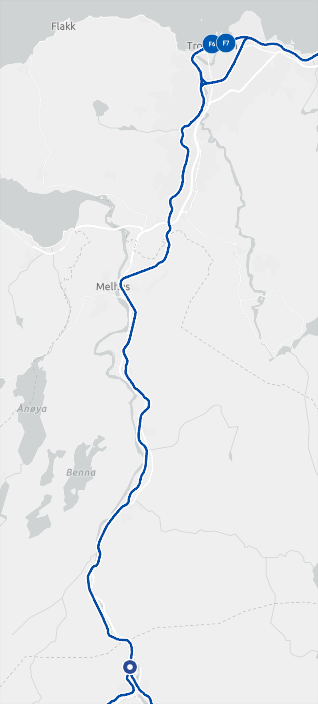
\includegraphics[scale=0.5]{figures/togkart.png}
    \caption{Map over train route from Trondheim to Støren}
    \label{fig:trainmap}
\end{figure}

\end{document}
